\documentclass[twoside]{book}

% Packages required by doxygen
\usepackage{fixltx2e}
\usepackage{calc}
\usepackage{doxygen}
\usepackage{graphicx}
\usepackage[utf8]{inputenc}
\usepackage{makeidx}
\usepackage{multicol}
\usepackage{multirow}
\PassOptionsToPackage{warn}{textcomp}
\usepackage{textcomp}
\usepackage[nointegrals]{wasysym}
\usepackage[table]{xcolor}

% Font selection
\usepackage[T1]{fontenc}
\usepackage{mathptmx}
\usepackage[scaled=.90]{helvet}
\usepackage{courier}
\usepackage{amssymb}
\usepackage{sectsty}
\renewcommand{\familydefault}{\sfdefault}
\allsectionsfont{%
  \fontseries{bc}\selectfont%
  \color{darkgray}%
}
\renewcommand{\DoxyLabelFont}{%
  \fontseries{bc}\selectfont%
  \color{darkgray}%
}
\newcommand{\+}{\discretionary{\mbox{\scriptsize$\hookleftarrow$}}{}{}}

% Page & text layout
\usepackage{geometry}
\geometry{%
  a4paper,%
  top=2.5cm,%
  bottom=2.5cm,%
  left=2.5cm,%
  right=2.5cm%
}
\tolerance=750
\hfuzz=15pt
\hbadness=750
\setlength{\emergencystretch}{15pt}
\setlength{\parindent}{0cm}
\setlength{\parskip}{0.2cm}
\makeatletter
\renewcommand{\paragraph}{%
  \@startsection{paragraph}{4}{0ex}{-1.0ex}{1.0ex}{%
    \normalfont\normalsize\bfseries\SS@parafont%
  }%
}
\renewcommand{\subparagraph}{%
  \@startsection{subparagraph}{5}{0ex}{-1.0ex}{1.0ex}{%
    \normalfont\normalsize\bfseries\SS@subparafont%
  }%
}
\makeatother

% Headers & footers
\usepackage{fancyhdr}
\pagestyle{fancyplain}
\fancyhead[LE]{\fancyplain{}{\bfseries\thepage}}
\fancyhead[CE]{\fancyplain{}{}}
\fancyhead[RE]{\fancyplain{}{\bfseries\leftmark}}
\fancyhead[LO]{\fancyplain{}{\bfseries\rightmark}}
\fancyhead[CO]{\fancyplain{}{}}
\fancyhead[RO]{\fancyplain{}{\bfseries\thepage}}
\fancyfoot[LE]{\fancyplain{}{}}
\fancyfoot[CE]{\fancyplain{}{}}
\fancyfoot[RE]{\fancyplain{}{\bfseries\scriptsize Generated on Sun Dec 18 2016 19\+:50\+:52 for X Runner by Doxygen }}
\fancyfoot[LO]{\fancyplain{}{\bfseries\scriptsize Generated on Sun Dec 18 2016 19\+:50\+:52 for X Runner by Doxygen }}
\fancyfoot[CO]{\fancyplain{}{}}
\fancyfoot[RO]{\fancyplain{}{}}
\renewcommand{\footrulewidth}{0.4pt}
\renewcommand{\chaptermark}[1]{%
  \markboth{#1}{}%
}
\renewcommand{\sectionmark}[1]{%
  \markright{\thesection\ #1}%
}

% Indices & bibliography
\usepackage{natbib}
\usepackage[titles]{tocloft}
\setcounter{tocdepth}{3}
\setcounter{secnumdepth}{5}
\makeindex

% Hyperlinks (required, but should be loaded last)
\usepackage{ifpdf}
\ifpdf
  \usepackage[pdftex,pagebackref=true]{hyperref}
\else
  \usepackage[ps2pdf,pagebackref=true]{hyperref}
\fi
\hypersetup{%
  colorlinks=true,%
  linkcolor=blue,%
  citecolor=blue,%
  unicode%
}

% Custom commands
\newcommand{\clearemptydoublepage}{%
  \newpage{\pagestyle{empty}\cleardoublepage}%
}


%===== C O N T E N T S =====

\begin{document}

% Titlepage & ToC
\hypersetup{pageanchor=false,
             bookmarks=true,
             bookmarksnumbered=true,
             pdfencoding=unicode
            }
\pagenumbering{roman}
\begin{titlepage}
\vspace*{7cm}
\begin{center}%
{\Large X Runner }\\
\vspace*{1cm}
{\large Generated by Doxygen 1.8.7}\\
\vspace*{0.5cm}
{\small Sun Dec 18 2016 19:50:52}\\
\end{center}
\end{titlepage}
\clearemptydoublepage
\tableofcontents
\clearemptydoublepage
\pagenumbering{arabic}
\hypersetup{pageanchor=true}

%--- Begin generated contents ---
\chapter{Hierarchical Index}
\section{Class Hierarchy}
This inheritance list is sorted roughly, but not completely, alphabetically\+:\begin{DoxyCompactList}
\item \contentsline{section}{Engine}{\pageref{classEngine}}{}
\item \contentsline{section}{Level\+\_\+\+Parser}{\pageref{classLevel__Parser}}{}
\item \contentsline{section}{Object}{\pageref{classObject}}{}
\begin{DoxyCompactList}
\item \contentsline{section}{Simulatable\+\_\+\+Object}{\pageref{classSimulatable__Object}}{}
\begin{DoxyCompactList}
\item \contentsline{section}{Movable\+\_\+\+Object}{\pageref{classMovable__Object}}{}
\begin{DoxyCompactList}
\item \contentsline{section}{Bird}{\pageref{classBird}}{}
\begin{DoxyCompactList}
\item \contentsline{section}{Boost\+\_\+\+Bird}{\pageref{classBoost__Bird}}{}
\item \contentsline{section}{Slow\+\_\+\+Bird}{\pageref{classSlow__Bird}}{}
\begin{DoxyCompactList}
\item \contentsline{section}{Bomb\+\_\+\+Bird}{\pageref{classBomb__Bird}}{}
\end{DoxyCompactList}
\end{DoxyCompactList}
\item \contentsline{section}{Gravitating\+\_\+\+Object}{\pageref{classGravitating__Object}}{}
\begin{DoxyCompactList}
\item \contentsline{section}{N\+F\+B\+B}{\pageref{classNFBB}}{}
\item \contentsline{section}{Player}{\pageref{classPlayer}}{}
\end{DoxyCompactList}
\end{DoxyCompactList}
\end{DoxyCompactList}
\end{DoxyCompactList}
\item \contentsline{section}{State}{\pageref{classState}}{}
\begin{DoxyCompactList}
\item \contentsline{section}{Game\+\_\+\+State}{\pageref{classGame__State}}{}
\item \contentsline{section}{Menu\+\_\+\+State}{\pageref{classMenu__State}}{}
\end{DoxyCompactList}
\end{DoxyCompactList}

\chapter{Class Index}
\section{Class List}
Here are the classes, structs, unions and interfaces with brief descriptions\+:\begin{DoxyCompactList}
\item\contentsline{section}{\hyperlink{structallow__remote__predicate}{allow\+\_\+remote\+\_\+predicate} }{\pageref{structallow__remote__predicate}}{}
\item\contentsline{section}{\hyperlink{structauto__deleter}{auto\+\_\+deleter$<$ T $>$} }{\pageref{structauto__deleter}}{}
\item\contentsline{section}{\hyperlink{structaxis__to__type}{axis\+\_\+to\+\_\+type$<$ N $>$} }{\pageref{structaxis__to__type}}{}
\item\contentsline{section}{\hyperlink{structxpath__parser_1_1binary__op__t}{xpath\+\_\+parser\+::binary\+\_\+op\+\_\+t} }{\pageref{structxpath__parser_1_1binary__op__t}}{}
\item\contentsline{section}{\hyperlink{classBird}{Bird} }{\pageref{classBird}}{}
\item\contentsline{section}{\hyperlink{classBomb__Bird}{Bomb\+\_\+\+Bird} }{\pageref{classBomb__Bird}}{}
\item\contentsline{section}{\hyperlink{classBoost__Bird}{Boost\+\_\+\+Bird} }{\pageref{classBoost__Bird}}{}
\item\contentsline{section}{\hyperlink{structdocument__order__comparator}{document\+\_\+order\+\_\+comparator} }{\pageref{structdocument__order__comparator}}{}
\item\contentsline{section}{\hyperlink{structduplicate__comparator}{duplicate\+\_\+comparator} }{\pageref{structduplicate__comparator}}{}
\item\contentsline{section}{\hyperlink{classEngine}{Engine} }{\pageref{classEngine}}{}
\item\contentsline{section}{\hyperlink{structequal__to}{equal\+\_\+to} }{\pageref{structequal__to}}{}
\item\contentsline{section}{\hyperlink{classGame__State}{Game\+\_\+\+State} }{\pageref{classGame__State}}{}
\item\contentsline{section}{\hyperlink{structgap}{gap} }{\pageref{structgap}}{}
\item\contentsline{section}{\hyperlink{classGravitating__Object}{Gravitating\+\_\+\+Object} }{\pageref{classGravitating__Object}}{}
\item\contentsline{section}{\hyperlink{structlatin1__decoder}{latin1\+\_\+decoder} }{\pageref{structlatin1__decoder}}{}
\item\contentsline{section}{\hyperlink{structlatin1__writer}{latin1\+\_\+writer} }{\pageref{structlatin1__writer}}{}
\item\contentsline{section}{\hyperlink{structless}{less} }{\pageref{structless}}{}
\item\contentsline{section}{\hyperlink{structless__equal}{less\+\_\+equal} }{\pageref{structless__equal}}{}
\item\contentsline{section}{\hyperlink{classLevel__Parser}{Level\+\_\+\+Parser} }{\pageref{classLevel__Parser}}{}
\item\contentsline{section}{\hyperlink{classMenu__State}{Menu\+\_\+\+State} }{\pageref{classMenu__State}}{}
\item\contentsline{section}{\hyperlink{classMovable__Object}{Movable\+\_\+\+Object} }{\pageref{classMovable__Object}}{}
\item\contentsline{section}{\hyperlink{structname__null__sentry}{name\+\_\+null\+\_\+sentry} }{\pageref{structname__null__sentry}}{}
\item\contentsline{section}{\hyperlink{structnamespace__uri__predicate}{namespace\+\_\+uri\+\_\+predicate} }{\pageref{structnamespace__uri__predicate}}{}
\item\contentsline{section}{\hyperlink{classNFBB}{N\+F\+B\+B} }{\pageref{classNFBB}}{}
\item\contentsline{section}{\hyperlink{structnot__equal__to}{not\+\_\+equal\+\_\+to} }{\pageref{structnot__equal__to}}{}
\item\contentsline{section}{\hyperlink{classObject}{Object} }{\pageref{classObject}}{}
\item\contentsline{section}{\hyperlink{structopt__false}{opt\+\_\+false} }{\pageref{structopt__false}}{}
\item\contentsline{section}{\hyperlink{structopt__true}{opt\+\_\+true} }{\pageref{structopt__true}}{}
\item\contentsline{section}{\hyperlink{classPlayer}{Player} }{\pageref{classPlayer}}{}
\item\contentsline{section}{\hyperlink{structboost_1_1range__const__iterator_3_01pugi_1_1xml__document_01_4}{boost\+::range\+\_\+const\+\_\+iterator$<$ pugi\+::xml\+\_\+document $>$} }{\pageref{structboost_1_1range__const__iterator_3_01pugi_1_1xml__document_01_4}}{}
\item\contentsline{section}{\hyperlink{structboost_1_1range__const__iterator_3_01pugi_1_1xml__node_01_4}{boost\+::range\+\_\+const\+\_\+iterator$<$ pugi\+::xml\+\_\+node $>$} }{\pageref{structboost_1_1range__const__iterator_3_01pugi_1_1xml__node_01_4}}{}
\item\contentsline{section}{\hyperlink{structboost_1_1range__mutable__iterator_3_01pugi_1_1xml__document_01_4}{boost\+::range\+\_\+mutable\+\_\+iterator$<$ pugi\+::xml\+\_\+document $>$} }{\pageref{structboost_1_1range__mutable__iterator_3_01pugi_1_1xml__document_01_4}}{}
\item\contentsline{section}{\hyperlink{structboost_1_1range__mutable__iterator_3_01pugi_1_1xml__node_01_4}{boost\+::range\+\_\+mutable\+\_\+iterator$<$ pugi\+::xml\+\_\+node $>$} }{\pageref{structboost_1_1range__mutable__iterator_3_01pugi_1_1xml__node_01_4}}{}
\item\contentsline{section}{\hyperlink{structsimple__walker}{simple\+\_\+walker} }{\pageref{structsimple__walker}}{}
\item\contentsline{section}{\hyperlink{classSimulatable__Object}{Simulatable\+\_\+\+Object} }{\pageref{classSimulatable__Object}}{}
\item\contentsline{section}{\hyperlink{classSlow__Bird}{Slow\+\_\+\+Bird} }{\pageref{classSlow__Bird}}{}
\item\contentsline{section}{\hyperlink{classState}{State} }{\pageref{classState}}{}
\item\contentsline{section}{\hyperlink{structstrconv__attribute__impl}{strconv\+\_\+attribute\+\_\+impl$<$ opt\+\_\+escape $>$} }{\pageref{structstrconv__attribute__impl}}{}
\item\contentsline{section}{\hyperlink{structstrconv__pcdata__impl}{strconv\+\_\+pcdata\+\_\+impl$<$ opt\+\_\+trim, opt\+\_\+eol, opt\+\_\+escape $>$} }{\pageref{structstrconv__pcdata__impl}}{}
\item\contentsline{section}{\hyperlink{structutf16__counter}{utf16\+\_\+counter} }{\pageref{structutf16__counter}}{}
\item\contentsline{section}{\hyperlink{structutf16__decoder}{utf16\+\_\+decoder$<$ opt\+\_\+swap $>$} }{\pageref{structutf16__decoder}}{}
\item\contentsline{section}{\hyperlink{structutf16__writer}{utf16\+\_\+writer} }{\pageref{structutf16__writer}}{}
\item\contentsline{section}{\hyperlink{structutf32__counter}{utf32\+\_\+counter} }{\pageref{structutf32__counter}}{}
\item\contentsline{section}{\hyperlink{structutf32__decoder}{utf32\+\_\+decoder$<$ opt\+\_\+swap $>$} }{\pageref{structutf32__decoder}}{}
\item\contentsline{section}{\hyperlink{structutf32__writer}{utf32\+\_\+writer} }{\pageref{structutf32__writer}}{}
\item\contentsline{section}{\hyperlink{structutf8__counter}{utf8\+\_\+counter} }{\pageref{structutf8__counter}}{}
\item\contentsline{section}{\hyperlink{structutf8__decoder}{utf8\+\_\+decoder} }{\pageref{structutf8__decoder}}{}
\item\contentsline{section}{\hyperlink{structutf8__writer}{utf8\+\_\+writer} }{\pageref{structutf8__writer}}{}
\item\contentsline{section}{\hyperlink{structwchar__decoder}{wchar\+\_\+decoder} }{\pageref{structwchar__decoder}}{}
\item\contentsline{section}{\hyperlink{structwchar__selector}{wchar\+\_\+selector$<$ size $>$} }{\pageref{structwchar__selector}}{}
\item\contentsline{section}{\hyperlink{structwchar__selector_3_012_01_4}{wchar\+\_\+selector$<$ 2 $>$} }{\pageref{structwchar__selector_3_012_01_4}}{}
\item\contentsline{section}{\hyperlink{structwchar__selector_3_014_01_4}{wchar\+\_\+selector$<$ 4 $>$} }{\pageref{structwchar__selector_3_014_01_4}}{}
\item\contentsline{section}{\hyperlink{structxml__allocator}{xml\+\_\+allocator} }{\pageref{structxml__allocator}}{}
\item\contentsline{section}{\hyperlink{classpugi_1_1xml__attribute}{pugi\+::xml\+\_\+attribute} }{\pageref{classpugi_1_1xml__attribute}}{}
\item\contentsline{section}{\hyperlink{classpugi_1_1xml__attribute__iterator}{pugi\+::xml\+\_\+attribute\+\_\+iterator} }{\pageref{classpugi_1_1xml__attribute__iterator}}{}
\item\contentsline{section}{\hyperlink{structpugi_1_1xml__attribute__struct}{pugi\+::xml\+\_\+attribute\+\_\+struct} }{\pageref{structpugi_1_1xml__attribute__struct}}{}
\item\contentsline{section}{\hyperlink{classxml__buffered__writer}{xml\+\_\+buffered\+\_\+writer} }{\pageref{classxml__buffered__writer}}{}
\item\contentsline{section}{\hyperlink{classpugi_1_1xml__document}{pugi\+::xml\+\_\+document} }{\pageref{classpugi_1_1xml__document}}{}
\item\contentsline{section}{\hyperlink{structxml__document__struct}{xml\+\_\+document\+\_\+struct} }{\pageref{structxml__document__struct}}{}
\item\contentsline{section}{\hyperlink{structxml__extra__buffer}{xml\+\_\+extra\+\_\+buffer} }{\pageref{structxml__extra__buffer}}{}
\item\contentsline{section}{\hyperlink{structxml__memory__management__function__storage}{xml\+\_\+memory\+\_\+management\+\_\+function\+\_\+storage$<$ T $>$} }{\pageref{structxml__memory__management__function__storage}}{}
\item\contentsline{section}{\hyperlink{structxml__memory__page}{xml\+\_\+memory\+\_\+page} }{\pageref{structxml__memory__page}}{}
\item\contentsline{section}{\hyperlink{structxml__memory__string__header}{xml\+\_\+memory\+\_\+string\+\_\+header} }{\pageref{structxml__memory__string__header}}{}
\item\contentsline{section}{\hyperlink{structxml__memory__writer}{xml\+\_\+memory\+\_\+writer} }{\pageref{structxml__memory__writer}}{}
\item\contentsline{section}{\hyperlink{classpugi_1_1xml__named__node__iterator}{pugi\+::xml\+\_\+named\+\_\+node\+\_\+iterator} }{\pageref{classpugi_1_1xml__named__node__iterator}}{}
\item\contentsline{section}{\hyperlink{classpugi_1_1xml__node}{pugi\+::xml\+\_\+node} }{\pageref{classpugi_1_1xml__node}}{}
\item\contentsline{section}{\hyperlink{classpugi_1_1xml__node__iterator}{pugi\+::xml\+\_\+node\+\_\+iterator} }{\pageref{classpugi_1_1xml__node__iterator}}{}
\item\contentsline{section}{\hyperlink{structpugi_1_1xml__node__struct}{pugi\+::xml\+\_\+node\+\_\+struct} }{\pageref{structpugi_1_1xml__node__struct}}{}
\item\contentsline{section}{\hyperlink{classpugi_1_1xml__object__range}{pugi\+::xml\+\_\+object\+\_\+range$<$ It $>$} }{\pageref{classpugi_1_1xml__object__range}}{}
\item\contentsline{section}{\hyperlink{structpugi_1_1xml__parse__result}{pugi\+::xml\+\_\+parse\+\_\+result} }{\pageref{structpugi_1_1xml__parse__result}}{}
\item\contentsline{section}{\hyperlink{structxml__parser}{xml\+\_\+parser} }{\pageref{structxml__parser}}{}
\item\contentsline{section}{\hyperlink{structxml__stream__chunk}{xml\+\_\+stream\+\_\+chunk$<$ T $>$} }{\pageref{structxml__stream__chunk}}{}
\item\contentsline{section}{\hyperlink{structxml__string__writer}{xml\+\_\+string\+\_\+writer} }{\pageref{structxml__string__writer}}{}
\item\contentsline{section}{\hyperlink{classpugi_1_1xml__text}{pugi\+::xml\+\_\+text} }{\pageref{classpugi_1_1xml__text}}{}
\item\contentsline{section}{\hyperlink{classpugi_1_1xml__tree__walker}{pugi\+::xml\+\_\+tree\+\_\+walker} }{\pageref{classpugi_1_1xml__tree__walker}}{}
\item\contentsline{section}{\hyperlink{classpugi_1_1xml__writer}{pugi\+::xml\+\_\+writer} }{\pageref{classpugi_1_1xml__writer}}{}
\item\contentsline{section}{\hyperlink{classpugi_1_1xml__writer__file}{pugi\+::xml\+\_\+writer\+\_\+file} }{\pageref{classpugi_1_1xml__writer__file}}{}
\item\contentsline{section}{\hyperlink{classpugi_1_1xml__writer__stream}{pugi\+::xml\+\_\+writer\+\_\+stream} }{\pageref{classpugi_1_1xml__writer__stream}}{}
\item\contentsline{section}{\hyperlink{classxpath__allocator}{xpath\+\_\+allocator} }{\pageref{classxpath__allocator}}{}
\item\contentsline{section}{\hyperlink{structxpath__allocator__capture}{xpath\+\_\+allocator\+\_\+capture} }{\pageref{structxpath__allocator__capture}}{}
\item\contentsline{section}{\hyperlink{classxpath__ast__node}{xpath\+\_\+ast\+\_\+node} }{\pageref{classxpath__ast__node}}{}
\item\contentsline{section}{\hyperlink{structxpath__context}{xpath\+\_\+context} }{\pageref{structxpath__context}}{}
\item\contentsline{section}{\hyperlink{classpugi_1_1xpath__exception}{pugi\+::xpath\+\_\+exception} }{\pageref{classpugi_1_1xpath__exception}}{}
\item\contentsline{section}{\hyperlink{classxpath__lexer}{xpath\+\_\+lexer} }{\pageref{classxpath__lexer}}{}
\item\contentsline{section}{\hyperlink{structxpath__lexer__string}{xpath\+\_\+lexer\+\_\+string} }{\pageref{structxpath__lexer__string}}{}
\item\contentsline{section}{\hyperlink{structxpath__memory__block}{xpath\+\_\+memory\+\_\+block} }{\pageref{structxpath__memory__block}}{}
\item\contentsline{section}{\hyperlink{classpugi_1_1xpath__node}{pugi\+::xpath\+\_\+node} }{\pageref{classpugi_1_1xpath__node}}{}
\item\contentsline{section}{\hyperlink{classpugi_1_1xpath__node__set}{pugi\+::xpath\+\_\+node\+\_\+set} }{\pageref{classpugi_1_1xpath__node__set}}{}
\item\contentsline{section}{\hyperlink{classxpath__node__set__raw}{xpath\+\_\+node\+\_\+set\+\_\+raw} }{\pageref{classxpath__node__set__raw}}{}
\item\contentsline{section}{\hyperlink{structpugi_1_1xpath__parse__result}{pugi\+::xpath\+\_\+parse\+\_\+result} }{\pageref{structpugi_1_1xpath__parse__result}}{}
\item\contentsline{section}{\hyperlink{structxpath__parser}{xpath\+\_\+parser} }{\pageref{structxpath__parser}}{}
\item\contentsline{section}{\hyperlink{classpugi_1_1xpath__query}{pugi\+::xpath\+\_\+query} }{\pageref{classpugi_1_1xpath__query}}{}
\item\contentsline{section}{\hyperlink{structxpath__query__impl}{xpath\+\_\+query\+\_\+impl} }{\pageref{structxpath__query__impl}}{}
\item\contentsline{section}{\hyperlink{structxpath__stack}{xpath\+\_\+stack} }{\pageref{structxpath__stack}}{}
\item\contentsline{section}{\hyperlink{structxpath__stack__data}{xpath\+\_\+stack\+\_\+data} }{\pageref{structxpath__stack__data}}{}
\item\contentsline{section}{\hyperlink{classxpath__string}{xpath\+\_\+string} }{\pageref{classxpath__string}}{}
\item\contentsline{section}{\hyperlink{classpugi_1_1xpath__variable}{pugi\+::xpath\+\_\+variable} }{\pageref{classpugi_1_1xpath__variable}}{}
\item\contentsline{section}{\hyperlink{structxpath__variable__boolean}{xpath\+\_\+variable\+\_\+boolean} }{\pageref{structxpath__variable__boolean}}{}
\item\contentsline{section}{\hyperlink{structxpath__variable__node__set}{xpath\+\_\+variable\+\_\+node\+\_\+set} }{\pageref{structxpath__variable__node__set}}{}
\item\contentsline{section}{\hyperlink{structxpath__variable__number}{xpath\+\_\+variable\+\_\+number} }{\pageref{structxpath__variable__number}}{}
\item\contentsline{section}{\hyperlink{classpugi_1_1xpath__variable__set}{pugi\+::xpath\+\_\+variable\+\_\+set} }{\pageref{classpugi_1_1xpath__variable__set}}{}
\item\contentsline{section}{\hyperlink{structxpath__variable__string}{xpath\+\_\+variable\+\_\+string} }{\pageref{structxpath__variable__string}}{}
\end{DoxyCompactList}

\chapter{Class Documentation}
\hypertarget{classBird}{\section{Bird Class Reference}
\label{classBird}\index{Bird@{Bird}}
}


Inheritance diagram for Bird\+:\nopagebreak
\begin{figure}[H]
\begin{center}
\leavevmode
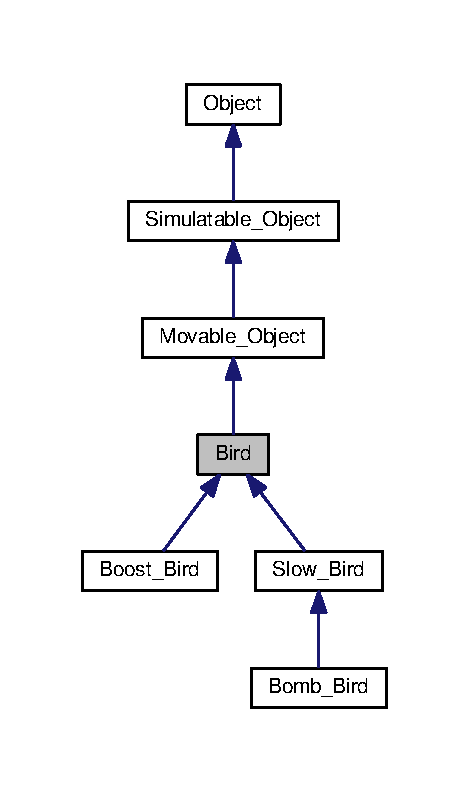
\includegraphics[width=226pt]{classBird__inherit__graph}
\end{center}
\end{figure}


Collaboration diagram for Bird\+:\nopagebreak
\begin{figure}[H]
\begin{center}
\leavevmode
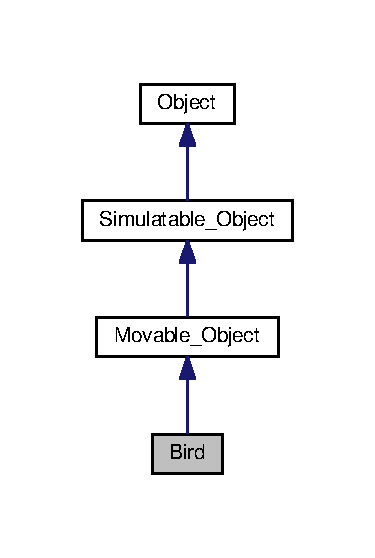
\includegraphics[width=180pt]{classBird__coll__graph}
\end{center}
\end{figure}
\subsection*{Public Member Functions}
\begin{DoxyCompactItemize}
\item 
\hyperlink{classBird_afe65295d7e648178245a1cd784924ecd}{Bird} (const sf\+::\+Vector2f \&, const sf\+::\+Vector2f \&, const std\+::string \&, const sf\+::\+Texture $\ast$, const float, const int, const float, const bool=false)
\begin{DoxyCompactList}\small\item\em \char`\"{}\+Constructor\char`\"{} \end{DoxyCompactList}\item 
virtual int \hyperlink{classBird_af2882ba302f03c5bdf5950cc21a39f66}{prepare\+\_\+simulate} (const float, const float) overridefinal
\begin{DoxyCompactList}\small\item\em \char`\"{}\+Prepares simulation of object\char`\"{} \end{DoxyCompactList}\end{DoxyCompactItemize}
\subsection*{Protected Member Functions}
\begin{DoxyCompactItemize}
\item 
\hypertarget{classBird_a3802ec1a4d2886ef8c95dd6d76038ab6}{virtual void {\bfseries handle\+\_\+moving\+\_\+collision} (const \hyperlink{classObject}{Object} $\ast$, const sf\+::\+Vector2f \&) overridefinal}\label{classBird_a3802ec1a4d2886ef8c95dd6d76038ab6}

\item 
\hypertarget{classBird_adbcfe9b09d3b828ce00982ec1aab9c6e}{virtual void {\bfseries handle\+\_\+static\+\_\+collision} (const \hyperlink{classObject}{Object} $\ast$)}\label{classBird_adbcfe9b09d3b828ce00982ec1aab9c6e}

\end{DoxyCompactItemize}
\subsection*{Protected Attributes}
\begin{DoxyCompactItemize}
\item 
\hypertarget{classBird_aad13ddaf4a6315ad3a2873e487cbc32b}{const float {\bfseries m\+\_\+speed}}\label{classBird_aad13ddaf4a6315ad3a2873e487cbc32b}

\item 
\hypertarget{classBird_a2e894d3d297ea72053ee319929c25f2c}{const float {\bfseries m\+\_\+cooldown}}\label{classBird_a2e894d3d297ea72053ee319929c25f2c}

\item 
\hypertarget{classBird_a2271962e5278b53dd7e600eea08465fc}{int {\bfseries m\+\_\+direction}}\label{classBird_a2271962e5278b53dd7e600eea08465fc}

\item 
\hypertarget{classBird_af212f094ae7b24978b494ef657ec9085}{sf\+::\+Clock {\bfseries m\+\_\+player\+\_\+clock}}\label{classBird_af212f094ae7b24978b494ef657ec9085}

\item 
\hypertarget{classBird_a0b43d6e0d01d780a18304731063897f6}{bool {\bfseries m\+\_\+player\+\_\+debuff} \{\}}\label{classBird_a0b43d6e0d01d780a18304731063897f6}

\end{DoxyCompactItemize}


\subsection{Constructor \& Destructor Documentation}
\hypertarget{classBird_afe65295d7e648178245a1cd784924ecd}{\index{Bird@{Bird}!Bird@{Bird}}
\index{Bird@{Bird}!Bird@{Bird}}
\subsubsection[{Bird}]{\setlength{\rightskip}{0pt plus 5cm}Bird\+::\+Bird (
\begin{DoxyParamCaption}
\item[{const sf\+::\+Vector2f \&}]{position, }
\item[{const sf\+::\+Vector2f \&}]{size, }
\item[{const std\+::string \&}]{type, }
\item[{const sf\+::\+Texture $\ast$}]{texture, }
\item[{const float}]{speed, }
\item[{const int}]{direction, }
\item[{const float}]{cooldown, }
\item[{const bool}]{solid = {\ttfamily false}}
\end{DoxyParamCaption}
)}}\label{classBird_afe65295d7e648178245a1cd784924ecd}


\char`\"{}\+Constructor\char`\"{} 


\begin{DoxyParams}{Parameters}
{\em position} & \char`\"{}\+Position of the object\char`\"{} \\
\hline
{\em size} & \char`\"{}\+Size of the object\char`\"{} \\
\hline
{\em type} & \char`\"{}\+Type of the object\char`\"{} \\
\hline
{\em texture} & \char`\"{}\+Texture of the object\char`\"{} \\
\hline
{\em speed} & \char`\"{}\+Speed of the object\char`\"{} \\
\hline
{\em direction} & \char`\"{}\+Direction of the object\char`\"{} \\
\hline
{\em cooldown} & \char`\"{}\+How long the objects opacity is 0.\+5\char`\"{} \\
\hline
{\em solid} & \char`\"{}\+If the object is solid\char`\"{} \\
\hline
\end{DoxyParams}


\subsection{Member Function Documentation}
\hypertarget{classBird_af2882ba302f03c5bdf5950cc21a39f66}{\index{Bird@{Bird}!prepare\+\_\+simulate@{prepare\+\_\+simulate}}
\index{prepare\+\_\+simulate@{prepare\+\_\+simulate}!Bird@{Bird}}
\subsubsection[{prepare\+\_\+simulate}]{\setlength{\rightskip}{0pt plus 5cm}int Bird\+::prepare\+\_\+simulate (
\begin{DoxyParamCaption}
\item[{const float}]{distance\+\_\+modifier, }
\item[{const float}]{}
\end{DoxyParamCaption}
)\hspace{0.3cm}{\ttfamily [final]}, {\ttfamily [override]}, {\ttfamily [virtual]}}}\label{classBird_af2882ba302f03c5bdf5950cc21a39f66}


\char`\"{}\+Prepares simulation of object\char`\"{} 


\begin{DoxyParams}{Parameters}
{\em distance\+\_\+modifier} & \char`\"{}\+Delta since last simulation-\/sequence\char`\"{} \\
\hline
{\em gravity\+\_\+constant} & \char`\"{}\+How much high the gravity is\char`\"{} \\
\hline
\end{DoxyParams}
\begin{DoxyReturn}{Returns}
\char`\"{}\+Simulation cycles required by this object this simulation-\/sequence\char`\"{} 
\end{DoxyReturn}


Implements \hyperlink{classSimulatable__Object_abe7c02fe250ef5be42011890d8a7b37b}{Simulatable\+\_\+\+Object}.



The documentation for this class was generated from the following files\+:\begin{DoxyCompactItemize}
\item 
objects/abstractish/bird.\+h\item 
objects/abstractish/bird.\+cc\end{DoxyCompactItemize}

\hypertarget{classBomb__Bird}{\section{Bomb\+\_\+\+Bird Class Reference}
\label{classBomb__Bird}\index{Bomb\+\_\+\+Bird@{Bomb\+\_\+\+Bird}}
}


Inheritance diagram for Bomb\+\_\+\+Bird\+:\nopagebreak
\begin{figure}[H]
\begin{center}
\leavevmode
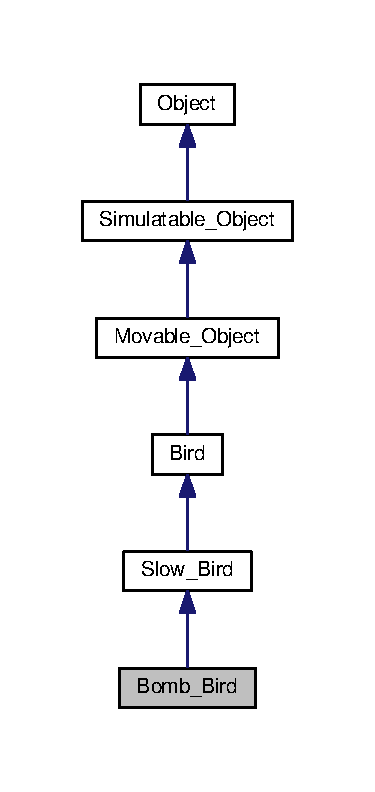
\includegraphics[width=180pt]{classBomb__Bird__inherit__graph}
\end{center}
\end{figure}


Collaboration diagram for Bomb\+\_\+\+Bird\+:\nopagebreak
\begin{figure}[H]
\begin{center}
\leavevmode
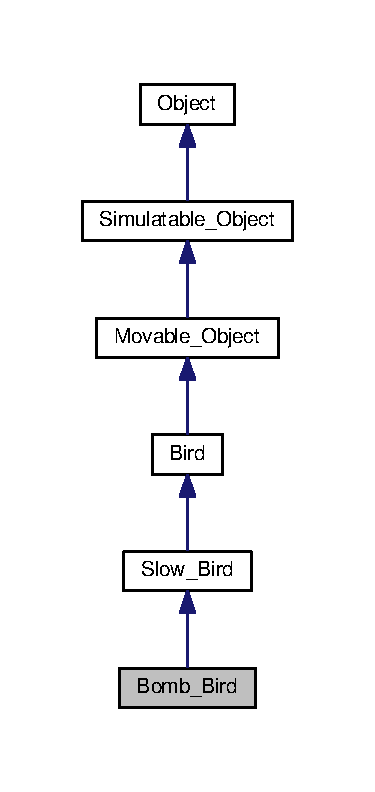
\includegraphics[width=180pt]{classBomb__Bird__coll__graph}
\end{center}
\end{figure}
\subsection*{Public Member Functions}
\begin{DoxyCompactItemize}
\item 
\hyperlink{classBomb__Bird_a920e7058e7cff86be951c2b9feede80e}{Bomb\+\_\+\+Bird} (const sf\+::\+Vector2f \&, const sf\+::\+Vector2f \&, const std\+::string \&, const sf\+::\+Texture $\ast$, const float, const int, const sf\+::\+Texture $\ast$)
\begin{DoxyCompactList}\small\item\em \char`\"{}\+Constructor\char`\"{} \end{DoxyCompactList}\item 
virtual std\+::vector$<$ \hyperlink{classObject}{Object} $\ast$ $>$ \hyperlink{classBomb__Bird_a610b4c68c560a6ac30375c177642e021}{simulate} (const int, const std\+::vector$<$ const \hyperlink{classObject}{Object} $\ast$ $>$ \&) overridefinal
\begin{DoxyCompactList}\small\item\em \char`\"{}\+Executes simulation of object\char`\"{} \end{DoxyCompactList}\end{DoxyCompactItemize}
\subsection*{Additional Inherited Members}


\subsection{Constructor \& Destructor Documentation}
\hypertarget{classBomb__Bird_a920e7058e7cff86be951c2b9feede80e}{\index{Bomb\+\_\+\+Bird@{Bomb\+\_\+\+Bird}!Bomb\+\_\+\+Bird@{Bomb\+\_\+\+Bird}}
\index{Bomb\+\_\+\+Bird@{Bomb\+\_\+\+Bird}!Bomb\+\_\+\+Bird@{Bomb\+\_\+\+Bird}}
\subsubsection[{Bomb\+\_\+\+Bird}]{\setlength{\rightskip}{0pt plus 5cm}Bomb\+\_\+\+Bird\+::\+Bomb\+\_\+\+Bird (
\begin{DoxyParamCaption}
\item[{const sf\+::\+Vector2f \&}]{position, }
\item[{const sf\+::\+Vector2f \&}]{size, }
\item[{const std\+::string \&}]{type, }
\item[{const sf\+::\+Texture $\ast$}]{texture, }
\item[{const float}]{speed, }
\item[{const int}]{direction, }
\item[{const sf\+::\+Texture $\ast$}]{nfbb\+\_\+texture}
\end{DoxyParamCaption}
)}}\label{classBomb__Bird_a920e7058e7cff86be951c2b9feede80e}


\char`\"{}\+Constructor\char`\"{} 


\begin{DoxyParams}{Parameters}
{\em position} & \char`\"{}\+Position of the object\char`\"{} \\
\hline
{\em size} & \char`\"{}\+Size of the object\char`\"{} \\
\hline
{\em type} & \char`\"{}\+Type of the object\char`\"{} \\
\hline
{\em texture} & \char`\"{}\+Texture of the object\char`\"{} \\
\hline
{\em speed} & \char`\"{}\+Speed of the object\char`\"{} \\
\hline
{\em direction} & \char`\"{}\+Direction of the object\char`\"{} \\
\hline
{\em nfbb\+\_\+texture} & \char`\"{}\+Texture of N\+F\+B\+B-\/objects spawned by the object\char`\"{} \\
\hline
\end{DoxyParams}


\subsection{Member Function Documentation}
\hypertarget{classBomb__Bird_a610b4c68c560a6ac30375c177642e021}{\index{Bomb\+\_\+\+Bird@{Bomb\+\_\+\+Bird}!simulate@{simulate}}
\index{simulate@{simulate}!Bomb\+\_\+\+Bird@{Bomb\+\_\+\+Bird}}
\subsubsection[{simulate}]{\setlength{\rightskip}{0pt plus 5cm}std\+::vector$<$ {\bf Object} $\ast$ $>$ Bomb\+\_\+\+Bird\+::simulate (
\begin{DoxyParamCaption}
\item[{const int}]{simulation\+\_\+cycles, }
\item[{const std\+::vector$<$ const {\bf Object} $\ast$ $>$ \&}]{objects}
\end{DoxyParamCaption}
)\hspace{0.3cm}{\ttfamily [final]}, {\ttfamily [override]}, {\ttfamily [virtual]}}}\label{classBomb__Bird_a610b4c68c560a6ac30375c177642e021}


\char`\"{}\+Executes simulation of object\char`\"{} 


\begin{DoxyParams}{Parameters}
{\em simulation\+\_\+cycles} & \char`\"{}\+Number simulation\+\_\+cycles the object will be subjected this simulation-\/sequence\char`\"{} \\
\hline
{\em objects} & \char`\"{}\+Objects to check for collision with\char`\"{} \\
\hline
\end{DoxyParams}
\begin{DoxyReturn}{Returns}
\char`\"{}\+New objects spawned by this object\char`\"{} 
\end{DoxyReturn}


Reimplemented from \hyperlink{classMovable__Object_ac267e0c945b558b0cf533d7fbe5ee7c3}{Movable\+\_\+\+Object}.



The documentation for this class was generated from the following files\+:\begin{DoxyCompactItemize}
\item 
objects/non\+\_\+abstract/bomb\+\_\+bird.\+h\item 
objects/non\+\_\+abstract/bomb\+\_\+bird.\+cc\end{DoxyCompactItemize}

\hypertarget{classBoost__Bird}{\section{Boost\+\_\+\+Bird Class Reference}
\label{classBoost__Bird}\index{Boost\+\_\+\+Bird@{Boost\+\_\+\+Bird}}
}


Inheritance diagram for Boost\+\_\+\+Bird\+:\nopagebreak
\begin{figure}[H]
\begin{center}
\leavevmode
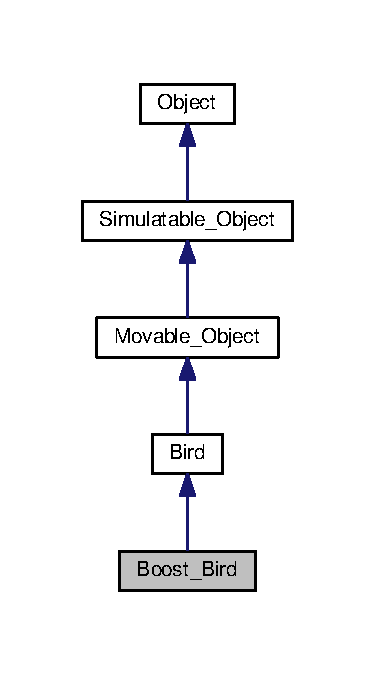
\includegraphics[width=180pt]{classBoost__Bird__inherit__graph}
\end{center}
\end{figure}


Collaboration diagram for Boost\+\_\+\+Bird\+:\nopagebreak
\begin{figure}[H]
\begin{center}
\leavevmode
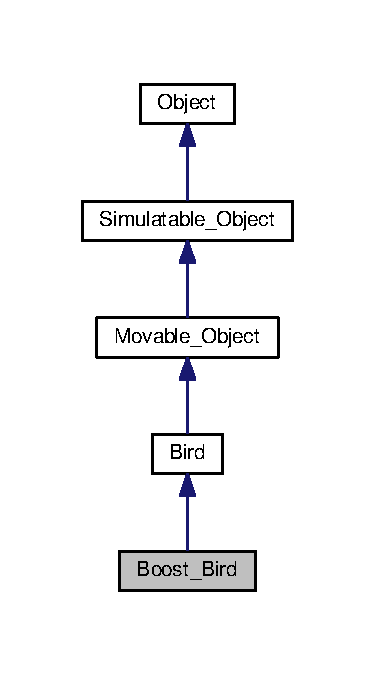
\includegraphics[width=180pt]{classBoost__Bird__coll__graph}
\end{center}
\end{figure}
\subsection*{Public Member Functions}
\begin{DoxyCompactItemize}
\item 
\hyperlink{classBoost__Bird_a03587afcb2e53cde2116d03d05f99846}{Boost\+\_\+\+Bird} (const sf\+::\+Vector2f \&, const sf\+::\+Vector2f \&, const std\+::string \&, const sf\+::\+Texture $\ast$, const float, const int)
\begin{DoxyCompactList}\small\item\em \char`\"{}\+Constructor\char`\"{} \end{DoxyCompactList}\end{DoxyCompactItemize}
\subsection*{Additional Inherited Members}


\subsection{Constructor \& Destructor Documentation}
\hypertarget{classBoost__Bird_a03587afcb2e53cde2116d03d05f99846}{\index{Boost\+\_\+\+Bird@{Boost\+\_\+\+Bird}!Boost\+\_\+\+Bird@{Boost\+\_\+\+Bird}}
\index{Boost\+\_\+\+Bird@{Boost\+\_\+\+Bird}!Boost\+\_\+\+Bird@{Boost\+\_\+\+Bird}}
\subsubsection[{Boost\+\_\+\+Bird}]{\setlength{\rightskip}{0pt plus 5cm}Boost\+\_\+\+Bird\+::\+Boost\+\_\+\+Bird (
\begin{DoxyParamCaption}
\item[{const sf\+::\+Vector2f \&}]{position, }
\item[{const sf\+::\+Vector2f \&}]{size, }
\item[{const std\+::string \&}]{type, }
\item[{const sf\+::\+Texture $\ast$}]{texture, }
\item[{const float}]{speed, }
\item[{const int}]{direction}
\end{DoxyParamCaption}
)}}\label{classBoost__Bird_a03587afcb2e53cde2116d03d05f99846}


\char`\"{}\+Constructor\char`\"{} 


\begin{DoxyParams}{Parameters}
{\em position} & \char`\"{}\+Position of the object\char`\"{} \\
\hline
{\em size} & \char`\"{}\+Size of the object\char`\"{} \\
\hline
{\em type} & \char`\"{}\+Type of the object\char`\"{} \\
\hline
{\em texture} & \char`\"{}\+Texture of the object\char`\"{} \\
\hline
{\em speed} & \char`\"{}\+Speed of the object\char`\"{} \\
\hline
{\em direction} & \char`\"{}\+Direction of the object\char`\"{} \\
\hline
\end{DoxyParams}


The documentation for this class was generated from the following files\+:\begin{DoxyCompactItemize}
\item 
objects/non\+\_\+abstract/boost\+\_\+bird.\+h\item 
objects/non\+\_\+abstract/boost\+\_\+bird.\+cc\end{DoxyCompactItemize}

\hypertarget{classEngine}{\section{Engine Class Reference}
\label{classEngine}\index{Engine@{Engine}}
}
\subsection*{Public Member Functions}
\begin{DoxyCompactItemize}
\item 
\hypertarget{classEngine_a8c98683b0a3aa28d8ab72a8bcd0d52f2}{\hyperlink{classEngine_a8c98683b0a3aa28d8ab72a8bcd0d52f2}{Engine} ()}\label{classEngine_a8c98683b0a3aa28d8ab72a8bcd0d52f2}

\begin{DoxyCompactList}\small\item\em \char`\"{}\+Constructor \+: creates State-\/objects and view,
        as well as setting the active-\/state and prepares it for simulation\char`\"{} \end{DoxyCompactList}\item 
\hypertarget{classEngine_a8ef7030a089ecb30bbfcb9e43094717a}{\hyperlink{classEngine_a8ef7030a089ecb30bbfcb9e43094717a}{$\sim$\+Engine} ()}\label{classEngine_a8ef7030a089ecb30bbfcb9e43094717a}

\begin{DoxyCompactList}\small\item\em \char`\"{}\+Destructor \+: frees resources owned by the Engine\char`\"{} \end{DoxyCompactList}\item 
void \hyperlink{classEngine_abedfd6c2327693f468b710bd79a9fe4c}{simulate} (sf\+::\+Render\+Window \&)
\begin{DoxyCompactList}\small\item\em \char`\"{}\+Simulates the active state, and, depending on the return value
       from the simulation, might change the active-\/state or close the window\char`\"{} \end{DoxyCompactList}\item 
void \hyperlink{classEngine_a4d9a19bdf6a13b84570e400acab6de6c}{render} (sf\+::\+Render\+Window \&)
\begin{DoxyCompactList}\small\item\em \char`\"{}draws all texturated objects and text objects in the active state\char`\"{} \end{DoxyCompactList}\end{DoxyCompactItemize}


\subsection{Member Function Documentation}
\hypertarget{classEngine_a4d9a19bdf6a13b84570e400acab6de6c}{\index{Engine@{Engine}!render@{render}}
\index{render@{render}!Engine@{Engine}}
\subsubsection[{render}]{\setlength{\rightskip}{0pt plus 5cm}void Engine\+::render (
\begin{DoxyParamCaption}
\item[{sf\+::\+Render\+Window \&}]{window}
\end{DoxyParamCaption}
)}}\label{classEngine_a4d9a19bdf6a13b84570e400acab6de6c}


\char`\"{}draws all texturated objects and text objects in the active state\char`\"{} 


\begin{DoxyParams}{Parameters}
{\em window} & \char`\"{}window draw on\char`\"{} \\
\hline
\end{DoxyParams}
\hypertarget{classEngine_abedfd6c2327693f468b710bd79a9fe4c}{\index{Engine@{Engine}!simulate@{simulate}}
\index{simulate@{simulate}!Engine@{Engine}}
\subsubsection[{simulate}]{\setlength{\rightskip}{0pt plus 5cm}void Engine\+::simulate (
\begin{DoxyParamCaption}
\item[{sf\+::\+Render\+Window \&}]{window}
\end{DoxyParamCaption}
)}}\label{classEngine_abedfd6c2327693f468b710bd79a9fe4c}


\char`\"{}\+Simulates the active state, and, depending on the return value
       from the simulation, might change the active-\/state or close the window\char`\"{} 


\begin{DoxyParams}{Parameters}
{\em window} & \char`\"{}window to close\char`\"{} \\
\hline
\end{DoxyParams}


The documentation for this class was generated from the following files\+:\begin{DoxyCompactItemize}
\item 
engine/engine.\+h\item 
engine/engine.\+cc\end{DoxyCompactItemize}

\hypertarget{classGame__State}{\section{Game\+\_\+\+State Class Reference}
\label{classGame__State}\index{Game\+\_\+\+State@{Game\+\_\+\+State}}
}


Inheritance diagram for Game\+\_\+\+State\+:\nopagebreak
\begin{figure}[H]
\begin{center}
\leavevmode
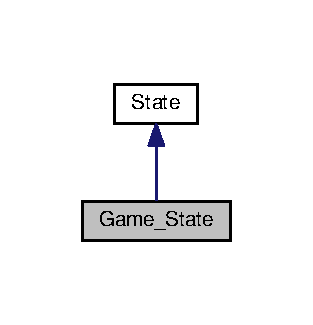
\includegraphics[width=150pt]{classGame__State__inherit__graph}
\end{center}
\end{figure}


Collaboration diagram for Game\+\_\+\+State\+:\nopagebreak
\begin{figure}[H]
\begin{center}
\leavevmode
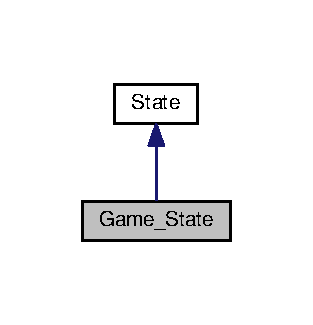
\includegraphics[width=150pt]{classGame__State__coll__graph}
\end{center}
\end{figure}
\subsection*{Public Member Functions}
\begin{DoxyCompactItemize}
\item 
\hypertarget{classGame__State_a8104ef051de61662ee5aef3f63c5d331}{\hyperlink{classGame__State_a8104ef051de61662ee5aef3f63c5d331}{Game\+\_\+\+State} ()}\label{classGame__State_a8104ef051de61662ee5aef3f63c5d331}

\begin{DoxyCompactList}\small\item\em \char`\"{}\+Constructor \+: loads all textures and fonts used in the state\char`\"{} \end{DoxyCompactList}\item 
\hypertarget{classGame__State_a9ad8826703bd8aff5bfeaba29b25e296}{void \hyperlink{classGame__State_a9ad8826703bd8aff5bfeaba29b25e296}{prepare\+\_\+simulate} () override}\label{classGame__State_a9ad8826703bd8aff5bfeaba29b25e296}

\begin{DoxyCompactList}\small\item\em \char`\"{}\+Resets the state and loads a new level into it with the help
        of the Level Parser class\char`\"{} \end{DoxyCompactList}\item 
int \hyperlink{classGame__State_ab45e81cb4c422cd23cd245cd3fb9c87f}{simulate} () override
\begin{DoxyCompactList}\small\item\em \char`\"{}\+Simulates each object in the state and performs actions on
        the state based on the result of the simulations\char`\"{} \end{DoxyCompactList}\item 
void \hyperlink{classGame__State_a1a24aa350628b7f3005e56c5efaadad7}{set\+\_\+view} (sf\+::\+View \&) override
\begin{DoxyCompactList}\small\item\em \char`\"{}\+Centers the view around the player\char`\"{} \end{DoxyCompactList}\end{DoxyCompactItemize}
\subsection*{Additional Inherited Members}


\subsection{Member Function Documentation}
\hypertarget{classGame__State_a1a24aa350628b7f3005e56c5efaadad7}{\index{Game\+\_\+\+State@{Game\+\_\+\+State}!set\+\_\+view@{set\+\_\+view}}
\index{set\+\_\+view@{set\+\_\+view}!Game\+\_\+\+State@{Game\+\_\+\+State}}
\subsubsection[{set\+\_\+view}]{\setlength{\rightskip}{0pt plus 5cm}void Game\+\_\+\+State\+::set\+\_\+view (
\begin{DoxyParamCaption}
\item[{sf\+::\+View \&}]{view}
\end{DoxyParamCaption}
)\hspace{0.3cm}{\ttfamily [override]}, {\ttfamily [virtual]}}}\label{classGame__State_a1a24aa350628b7f3005e56c5efaadad7}


\char`\"{}\+Centers the view around the player\char`\"{} 


\begin{DoxyParams}{Parameters}
{\em view} & \char`\"{}\+View to perform action on\char`\"{} \\
\hline
\end{DoxyParams}


Implements \hyperlink{classState}{State}.

\hypertarget{classGame__State_ab45e81cb4c422cd23cd245cd3fb9c87f}{\index{Game\+\_\+\+State@{Game\+\_\+\+State}!simulate@{simulate}}
\index{simulate@{simulate}!Game\+\_\+\+State@{Game\+\_\+\+State}}
\subsubsection[{simulate}]{\setlength{\rightskip}{0pt plus 5cm}int Game\+\_\+\+State\+::simulate (
\begin{DoxyParamCaption}
{}
\end{DoxyParamCaption}
)\hspace{0.3cm}{\ttfamily [override]}, {\ttfamily [virtual]}}}\label{classGame__State_ab45e81cb4c422cd23cd245cd3fb9c87f}


\char`\"{}\+Simulates each object in the state and performs actions on
        the state based on the result of the simulations\char`\"{} 

\begin{DoxyReturn}{Returns}
\char`\"{}\+An integer representing the next action to be taken by the Engine object\char`\"{} 
\end{DoxyReturn}


Implements \hyperlink{classState}{State}.



The documentation for this class was generated from the following files\+:\begin{DoxyCompactItemize}
\item 
states/non\+\_\+abstract/game\+\_\+state.\+h\item 
states/non\+\_\+abstract/game\+\_\+state.\+cc\end{DoxyCompactItemize}

\hypertarget{classGravitating__Object}{\section{Gravitating\+\_\+\+Object Class Reference}
\label{classGravitating__Object}\index{Gravitating\+\_\+\+Object@{Gravitating\+\_\+\+Object}}
}


Inheritance diagram for Gravitating\+\_\+\+Object\+:\nopagebreak
\begin{figure}[H]
\begin{center}
\leavevmode
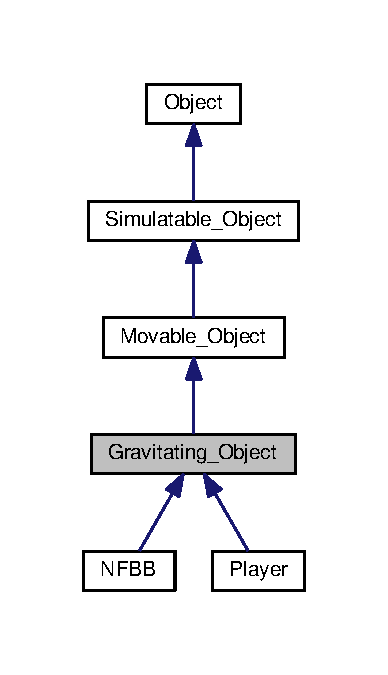
\includegraphics[width=186pt]{classGravitating__Object__inherit__graph}
\end{center}
\end{figure}


Collaboration diagram for Gravitating\+\_\+\+Object\+:\nopagebreak
\begin{figure}[H]
\begin{center}
\leavevmode
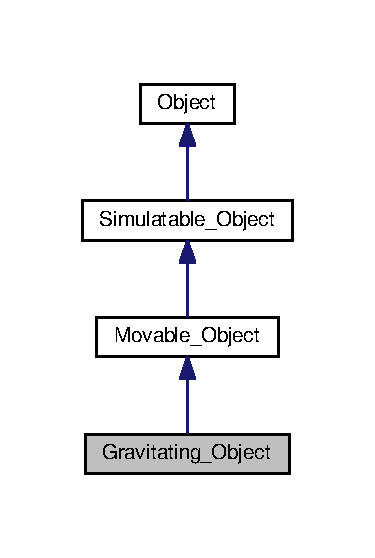
\includegraphics[width=180pt]{classGravitating__Object__coll__graph}
\end{center}
\end{figure}
\subsection*{Public Member Functions}
\begin{DoxyCompactItemize}
\item 
\hyperlink{classGravitating__Object_a7319a97eb2d84afbe66c5e0040bd3973}{Gravitating\+\_\+\+Object} (const sf\+::\+Vector2f \&, const sf\+::\+Vector2f \&, const std\+::string \&, const bool=false, const sf\+::\+Texture $\ast$=nullptr)
\begin{DoxyCompactList}\small\item\em \char`\"{}\+Constructor\char`\"{} \end{DoxyCompactList}\item 
int \hyperlink{classGravitating__Object_a187404d6df6ff16a86a33a3f4a8aab85}{prepare\+\_\+simulate} (const float, const float)
\begin{DoxyCompactList}\small\item\em \char`\"{}\+Prepares simulation of object\char`\"{} \end{DoxyCompactList}\end{DoxyCompactItemize}
\subsection*{Protected Member Functions}
\begin{DoxyCompactItemize}
\item 
\hypertarget{classGravitating__Object_ad059f059b3699edb3edff11fdd7fba29}{virtual void {\bfseries handle\+\_\+moving\+\_\+collision} (const \hyperlink{classObject}{Object} $\ast$, const sf\+::\+Vector2f \&) override}\label{classGravitating__Object_ad059f059b3699edb3edff11fdd7fba29}

\end{DoxyCompactItemize}
\subsection*{Protected Attributes}
\begin{DoxyCompactItemize}
\item 
\hypertarget{classGravitating__Object_abda4e488702c931d99b47785db6be33b}{sf\+::\+Clock {\bfseries m\+\_\+gravity\+\_\+clock}}\label{classGravitating__Object_abda4e488702c931d99b47785db6be33b}

\end{DoxyCompactItemize}


\subsection{Constructor \& Destructor Documentation}
\hypertarget{classGravitating__Object_a7319a97eb2d84afbe66c5e0040bd3973}{\index{Gravitating\+\_\+\+Object@{Gravitating\+\_\+\+Object}!Gravitating\+\_\+\+Object@{Gravitating\+\_\+\+Object}}
\index{Gravitating\+\_\+\+Object@{Gravitating\+\_\+\+Object}!Gravitating\+\_\+\+Object@{Gravitating\+\_\+\+Object}}
\subsubsection[{Gravitating\+\_\+\+Object}]{\setlength{\rightskip}{0pt plus 5cm}Gravitating\+\_\+\+Object\+::\+Gravitating\+\_\+\+Object (
\begin{DoxyParamCaption}
\item[{const sf\+::\+Vector2f \&}]{position, }
\item[{const sf\+::\+Vector2f \&}]{size, }
\item[{const std\+::string \&}]{type, }
\item[{const bool}]{solid = {\ttfamily false}, }
\item[{const sf\+::\+Texture $\ast$}]{texture = {\ttfamily nullptr}}
\end{DoxyParamCaption}
)}}\label{classGravitating__Object_a7319a97eb2d84afbe66c5e0040bd3973}


\char`\"{}\+Constructor\char`\"{} 


\begin{DoxyParams}{Parameters}
{\em position} & \char`\"{}\+Position of the object\char`\"{} \\
\hline
{\em size} & \char`\"{}\+Size of the object\char`\"{} \\
\hline
{\em type} & \char`\"{}\+Type of the object\char`\"{} \\
\hline
{\em solid} & \char`\"{}\+If the object is solid\char`\"{} \\
\hline
{\em texture} & \char`\"{}\+Texture of the object\char`\"{}" \\
\hline
\end{DoxyParams}


\subsection{Member Function Documentation}
\hypertarget{classGravitating__Object_a187404d6df6ff16a86a33a3f4a8aab85}{\index{Gravitating\+\_\+\+Object@{Gravitating\+\_\+\+Object}!prepare\+\_\+simulate@{prepare\+\_\+simulate}}
\index{prepare\+\_\+simulate@{prepare\+\_\+simulate}!Gravitating\+\_\+\+Object@{Gravitating\+\_\+\+Object}}
\subsubsection[{prepare\+\_\+simulate}]{\setlength{\rightskip}{0pt plus 5cm}int Gravitating\+\_\+\+Object\+::prepare\+\_\+simulate (
\begin{DoxyParamCaption}
\item[{const float}]{distance\+\_\+modifier, }
\item[{const float}]{gravity\+\_\+constant}
\end{DoxyParamCaption}
)\hspace{0.3cm}{\ttfamily [virtual]}}}\label{classGravitating__Object_a187404d6df6ff16a86a33a3f4a8aab85}


\char`\"{}\+Prepares simulation of object\char`\"{} 


\begin{DoxyParams}{Parameters}
{\em distance\+\_\+modifier} & \char`\"{}\+Delta since last simulation-\/sequence\char`\"{} \\
\hline
{\em gravity\+\_\+constant} & \char`\"{}\+How much high the gravity is\char`\"{} \\
\hline
\end{DoxyParams}
\begin{DoxyReturn}{Returns}
\char`\"{}\+Simulation cycles required by this object this simulation-\/sequence\char`\"{} 
\end{DoxyReturn}


Implements \hyperlink{classSimulatable__Object_abe7c02fe250ef5be42011890d8a7b37b}{Simulatable\+\_\+\+Object}.



Reimplemented in \hyperlink{classPlayer_a1480bbfb767687380ad6a2bf294cdcc8}{Player}.



The documentation for this class was generated from the following files\+:\begin{DoxyCompactItemize}
\item 
objects/abstractish/gravitating\+\_\+object.\+h\item 
objects/abstractish/gravitating\+\_\+object.\+cc\end{DoxyCompactItemize}

\hypertarget{classLevel__Parser}{\section{Level\+\_\+\+Parser Class Reference}
\label{classLevel__Parser}\index{Level\+\_\+\+Parser@{Level\+\_\+\+Parser}}
}
\subsection*{Public Member Functions}
\begin{DoxyCompactItemize}
\item 
\hyperlink{classLevel__Parser_ac1e8138a19ac3d284010c693e5ca446c}{Level\+\_\+\+Parser} (const std\+::string \&)
\begin{DoxyCompactList}\small\item\em \char`\"{}\+Constructor\char`\"{} \end{DoxyCompactList}\item 
std\+::vector$<$ \hyperlink{classObject}{Object} $\ast$ $>$ \hyperlink{classLevel__Parser_af3206216900aae52b79289c3f75c1e32}{get\+\_\+objects} (const std\+::unordered\+\_\+map$<$ std\+::string, sf\+::\+Texture $\ast$ $>$ \&) const 
\begin{DoxyCompactList}\small\item\em \char`\"{}\+Creates and returns all objects in loaded file\char`\"{} \end{DoxyCompactList}\end{DoxyCompactItemize}


\subsection{Constructor \& Destructor Documentation}
\hypertarget{classLevel__Parser_ac1e8138a19ac3d284010c693e5ca446c}{\index{Level\+\_\+\+Parser@{Level\+\_\+\+Parser}!Level\+\_\+\+Parser@{Level\+\_\+\+Parser}}
\index{Level\+\_\+\+Parser@{Level\+\_\+\+Parser}!Level\+\_\+\+Parser@{Level\+\_\+\+Parser}}
\subsubsection[{Level\+\_\+\+Parser}]{\setlength{\rightskip}{0pt plus 5cm}Level\+\_\+\+Parser\+::\+Level\+\_\+\+Parser (
\begin{DoxyParamCaption}
\item[{const std\+::string \&}]{path}
\end{DoxyParamCaption}
)}}\label{classLevel__Parser_ac1e8138a19ac3d284010c693e5ca446c}


\char`\"{}\+Constructor\char`\"{} 


\begin{DoxyParams}{Parameters}
{\em path} & \char`\"{}\+Path to xml-\/file to load\char`\"{} \\
\hline
\end{DoxyParams}


\subsection{Member Function Documentation}
\hypertarget{classLevel__Parser_af3206216900aae52b79289c3f75c1e32}{\index{Level\+\_\+\+Parser@{Level\+\_\+\+Parser}!get\+\_\+objects@{get\+\_\+objects}}
\index{get\+\_\+objects@{get\+\_\+objects}!Level\+\_\+\+Parser@{Level\+\_\+\+Parser}}
\subsubsection[{get\+\_\+objects}]{\setlength{\rightskip}{0pt plus 5cm}std\+::vector$<$ {\bf Object} $\ast$ $>$ Level\+\_\+\+Parser\+::get\+\_\+objects (
\begin{DoxyParamCaption}
\item[{const std\+::unordered\+\_\+map$<$ std\+::string, sf\+::\+Texture $\ast$ $>$ \&}]{textures}
\end{DoxyParamCaption}
) const}}\label{classLevel__Parser_af3206216900aae52b79289c3f75c1e32}


\char`\"{}\+Creates and returns all objects in loaded file\char`\"{} 


\begin{DoxyParams}{Parameters}
{\em textures} & \char`\"{}\+Textures to create objects with\char`\"{} \\
\hline
\end{DoxyParams}
\begin{DoxyReturn}{Returns}
\char`\"{}\+All objects in loaded file\char`\"{} 
\end{DoxyReturn}


The documentation for this class was generated from the following files\+:\begin{DoxyCompactItemize}
\item 
level\+\_\+parser/level\+\_\+parser.\+h\item 
level\+\_\+parser/level\+\_\+parser.\+cc\end{DoxyCompactItemize}

\hypertarget{classMenu__State}{\section{Menu\+\_\+\+State Class Reference}
\label{classMenu__State}\index{Menu\+\_\+\+State@{Menu\+\_\+\+State}}
}


Inheritance diagram for Menu\+\_\+\+State\+:\nopagebreak
\begin{figure}[H]
\begin{center}
\leavevmode
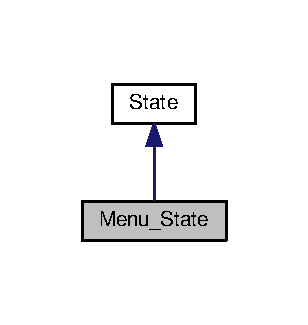
\includegraphics[width=148pt]{classMenu__State__inherit__graph}
\end{center}
\end{figure}


Collaboration diagram for Menu\+\_\+\+State\+:\nopagebreak
\begin{figure}[H]
\begin{center}
\leavevmode
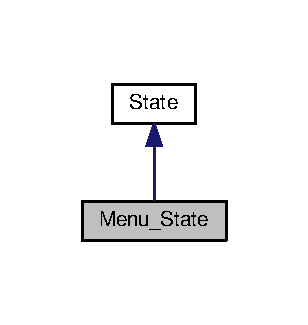
\includegraphics[width=148pt]{classMenu__State__coll__graph}
\end{center}
\end{figure}
\subsection*{Public Member Functions}
\begin{DoxyCompactItemize}
\item 
\hypertarget{classMenu__State_abcb7829ec9a970e44efa5c235e988cfb}{\hyperlink{classMenu__State_abcb7829ec9a970e44efa5c235e988cfb}{Menu\+\_\+\+State} ()}\label{classMenu__State_abcb7829ec9a970e44efa5c235e988cfb}

\begin{DoxyCompactList}\small\item\em \char`\"{}\+Constructor \+: loads all textures and fonts used in the state\char`\"{} \end{DoxyCompactList}\item 
\hypertarget{classMenu__State_a654017b2f4425a4d2e2827bc35c113eb}{void \hyperlink{classMenu__State_a654017b2f4425a4d2e2827bc35c113eb}{prepare\+\_\+simulate} () override}\label{classMenu__State_a654017b2f4425a4d2e2827bc35c113eb}

\begin{DoxyCompactList}\small\item\em \char`\"{}\+Resets the state and loads a new level into it with the help
        of the Level Parser class\char`\"{} \end{DoxyCompactList}\item 
int \hyperlink{classMenu__State_a8c8cd24b56f7123085195accaa6e1a48}{simulate} () override
\begin{DoxyCompactList}\small\item\em \char`\"{}\+Simulates each object in the state and performs actions on
        the state based on the result of the simulations\char`\"{} \end{DoxyCompactList}\item 
void \hyperlink{classMenu__State_a7a65c4db5146110cb6597b69226c4f1b}{set\+\_\+view} (sf\+::\+View \&) override
\begin{DoxyCompactList}\small\item\em \char`\"{}\+Centers the view around the player\char`\"{} \end{DoxyCompactList}\end{DoxyCompactItemize}
\subsection*{Additional Inherited Members}


\subsection{Member Function Documentation}
\hypertarget{classMenu__State_a7a65c4db5146110cb6597b69226c4f1b}{\index{Menu\+\_\+\+State@{Menu\+\_\+\+State}!set\+\_\+view@{set\+\_\+view}}
\index{set\+\_\+view@{set\+\_\+view}!Menu\+\_\+\+State@{Menu\+\_\+\+State}}
\subsubsection[{set\+\_\+view}]{\setlength{\rightskip}{0pt plus 5cm}void Menu\+\_\+\+State\+::set\+\_\+view (
\begin{DoxyParamCaption}
\item[{sf\+::\+View \&}]{view}
\end{DoxyParamCaption}
)\hspace{0.3cm}{\ttfamily [override]}, {\ttfamily [virtual]}}}\label{classMenu__State_a7a65c4db5146110cb6597b69226c4f1b}


\char`\"{}\+Centers the view around the player\char`\"{} 


\begin{DoxyParams}{Parameters}
{\em view} & \char`\"{}\+View to perform action on\char`\"{} \\
\hline
\end{DoxyParams}


Implements \hyperlink{classState}{State}.

\hypertarget{classMenu__State_a8c8cd24b56f7123085195accaa6e1a48}{\index{Menu\+\_\+\+State@{Menu\+\_\+\+State}!simulate@{simulate}}
\index{simulate@{simulate}!Menu\+\_\+\+State@{Menu\+\_\+\+State}}
\subsubsection[{simulate}]{\setlength{\rightskip}{0pt plus 5cm}int Menu\+\_\+\+State\+::simulate (
\begin{DoxyParamCaption}
{}
\end{DoxyParamCaption}
)\hspace{0.3cm}{\ttfamily [override]}, {\ttfamily [virtual]}}}\label{classMenu__State_a8c8cd24b56f7123085195accaa6e1a48}


\char`\"{}\+Simulates each object in the state and performs actions on
        the state based on the result of the simulations\char`\"{} 

\begin{DoxyReturn}{Returns}
\char`\"{}\+An integer representing the next action to be taken by the Engine object\char`\"{} 
\end{DoxyReturn}


Implements \hyperlink{classState}{State}.



The documentation for this class was generated from the following files\+:\begin{DoxyCompactItemize}
\item 
states/non\+\_\+abstract/menu\+\_\+state.\+h\item 
states/non\+\_\+abstract/menu\+\_\+state.\+cc\end{DoxyCompactItemize}

\hypertarget{classMovable__Object}{\section{Movable\+\_\+\+Object Class Reference}
\label{classMovable__Object}\index{Movable\+\_\+\+Object@{Movable\+\_\+\+Object}}
}


Inheritance diagram for Movable\+\_\+\+Object\+:\nopagebreak
\begin{figure}[H]
\begin{center}
\leavevmode
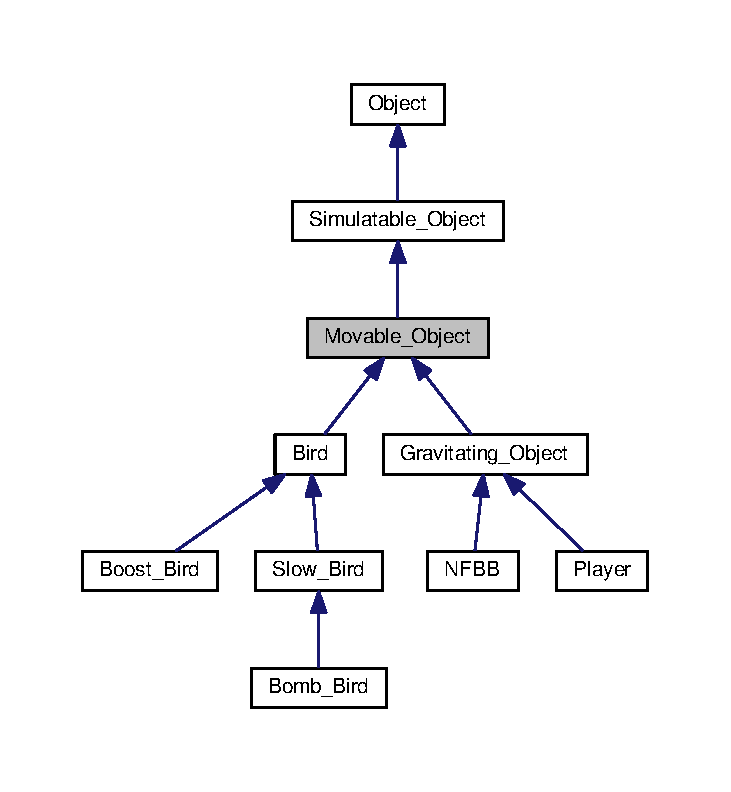
\includegraphics[width=350pt]{classMovable__Object__inherit__graph}
\end{center}
\end{figure}


Collaboration diagram for Movable\+\_\+\+Object\+:\nopagebreak
\begin{figure}[H]
\begin{center}
\leavevmode
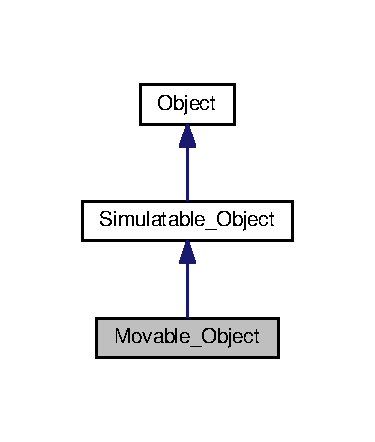
\includegraphics[width=180pt]{classMovable__Object__coll__graph}
\end{center}
\end{figure}
\subsection*{Public Member Functions}
\begin{DoxyCompactItemize}
\item 
\hyperlink{classMovable__Object_a7ef80ffc751a380e9c0beb7d4f0da9ce}{Movable\+\_\+\+Object} (const sf\+::\+Vector2f \&, const sf\+::\+Vector2f \&, const std\+::string \&, const bool=false, const sf\+::\+Texture $\ast$=nullptr)
\begin{DoxyCompactList}\small\item\em \char`\"{}\+Constructor\char`\"{} \end{DoxyCompactList}\item 
int \hyperlink{classMovable__Object_aed1d50e30dc96faea3250bee8b4af227}{prepare\+\_\+simulate} (const float)
\begin{DoxyCompactList}\small\item\em \char`\"{}\+Prepares simulation of object\char`\"{} \end{DoxyCompactList}\item 
virtual std\+::vector$<$ \hyperlink{classObject}{Object} $\ast$ $>$ \hyperlink{classMovable__Object_ac267e0c945b558b0cf533d7fbe5ee7c3}{simulate} (const int, const std\+::vector$<$ const \hyperlink{classObject}{Object} $\ast$ $>$ \&) override
\begin{DoxyCompactList}\small\item\em \char`\"{}\+Executes simulation of object\char`\"{} \end{DoxyCompactList}\item 
virtual void \hyperlink{classMovable__Object_ac9111a729082cd46a913e1877a57a930}{end\+\_\+simulate} (const std\+::vector$<$ const \hyperlink{classObject}{Object} $\ast$ $>$ \&objects) override
\begin{DoxyCompactList}\small\item\em \char`\"{}\+Executes end-\/of-\/simulation logic of object\char`\"{} \end{DoxyCompactList}\end{DoxyCompactItemize}
\subsection*{Protected Member Functions}
\begin{DoxyCompactItemize}
\item 
\hypertarget{classMovable__Object_a909989f83255795f755742be6db62713}{virtual void {\bfseries handle\+\_\+moving\+\_\+collision} (const \hyperlink{classObject}{Object} $\ast$, const sf\+::\+Vector2f \&)}\label{classMovable__Object_a909989f83255795f755742be6db62713}

\item 
\hypertarget{classMovable__Object_a7091c50aa4cd1438424737441e9ff72a}{virtual void {\bfseries collision\+\_\+state\+\_\+cleanup} ()}\label{classMovable__Object_a7091c50aa4cd1438424737441e9ff72a}

\item 
\hypertarget{classMovable__Object_a1d92a4bbc7c741bf3d1c65004eab2adb}{virtual void {\bfseries handle\+\_\+static\+\_\+collision} (const \hyperlink{classObject}{Object} $\ast$)}\label{classMovable__Object_a1d92a4bbc7c741bf3d1c65004eab2adb}

\item 
\hypertarget{classMovable__Object_a71916586f5f73c836568503dcd7b0eb7}{virtual void {\bfseries handle\+\_\+end\+\_\+collision} ()}\label{classMovable__Object_a71916586f5f73c836568503dcd7b0eb7}

\end{DoxyCompactItemize}
\subsection*{Protected Attributes}
\begin{DoxyCompactItemize}
\item 
\hypertarget{classMovable__Object_a3824126abcb82e10d65c0427ac291ef4}{sf\+::\+Vector2f {\bfseries m\+\_\+distance}}\label{classMovable__Object_a3824126abcb82e10d65c0427ac291ef4}

\item 
\hypertarget{classMovable__Object_a00d1c3d1f5cb644a9d9de84128de136f}{bool {\bfseries m\+\_\+ground\+\_\+collision} \{\}}\label{classMovable__Object_a00d1c3d1f5cb644a9d9de84128de136f}

\item 
\hypertarget{classMovable__Object_aa491f8684b9fa3d4d81047de1ad644ee}{bool {\bfseries m\+\_\+roof\+\_\+collision} \{\}}\label{classMovable__Object_aa491f8684b9fa3d4d81047de1ad644ee}

\item 
\hypertarget{classMovable__Object_aacdedf600c68dbfaa756484c39ae9229}{bool {\bfseries m\+\_\+wall\+\_\+collision} \{\}}\label{classMovable__Object_aacdedf600c68dbfaa756484c39ae9229}

\end{DoxyCompactItemize}


\subsection{Constructor \& Destructor Documentation}
\hypertarget{classMovable__Object_a7ef80ffc751a380e9c0beb7d4f0da9ce}{\index{Movable\+\_\+\+Object@{Movable\+\_\+\+Object}!Movable\+\_\+\+Object@{Movable\+\_\+\+Object}}
\index{Movable\+\_\+\+Object@{Movable\+\_\+\+Object}!Movable\+\_\+\+Object@{Movable\+\_\+\+Object}}
\subsubsection[{Movable\+\_\+\+Object}]{\setlength{\rightskip}{0pt plus 5cm}Movable\+\_\+\+Object\+::\+Movable\+\_\+\+Object (
\begin{DoxyParamCaption}
\item[{const sf\+::\+Vector2f \&}]{position, }
\item[{const sf\+::\+Vector2f \&}]{size, }
\item[{const std\+::string \&}]{type, }
\item[{const bool}]{solid = {\ttfamily false}, }
\item[{const sf\+::\+Texture $\ast$}]{texture = {\ttfamily nullptr}}
\end{DoxyParamCaption}
)}}\label{classMovable__Object_a7ef80ffc751a380e9c0beb7d4f0da9ce}


\char`\"{}\+Constructor\char`\"{} 


\begin{DoxyParams}{Parameters}
{\em position} & \char`\"{}\+Position of the object\char`\"{} \\
\hline
{\em size} & \char`\"{}\+Size of the object\char`\"{} \\
\hline
{\em type} & \char`\"{}\+Type of the object\char`\"{} \\
\hline
{\em solid} & \char`\"{}\+If the object is solid\char`\"{} \\
\hline
{\em texture} & \char`\"{}\+Texture of the object\char`\"{}" \\
\hline
\end{DoxyParams}


\subsection{Member Function Documentation}
\hypertarget{classMovable__Object_ac9111a729082cd46a913e1877a57a930}{\index{Movable\+\_\+\+Object@{Movable\+\_\+\+Object}!end\+\_\+simulate@{end\+\_\+simulate}}
\index{end\+\_\+simulate@{end\+\_\+simulate}!Movable\+\_\+\+Object@{Movable\+\_\+\+Object}}
\subsubsection[{end\+\_\+simulate}]{\setlength{\rightskip}{0pt plus 5cm}void Movable\+\_\+\+Object\+::end\+\_\+simulate (
\begin{DoxyParamCaption}
\item[{const std\+::vector$<$ const {\bf Object} $\ast$ $>$ \&}]{objects}
\end{DoxyParamCaption}
)\hspace{0.3cm}{\ttfamily [override]}, {\ttfamily [virtual]}}}\label{classMovable__Object_ac9111a729082cd46a913e1877a57a930}


\char`\"{}\+Executes end-\/of-\/simulation logic of object\char`\"{} 


\begin{DoxyParams}{Parameters}
{\em objects} & \char`\"{}\+Objects to check for collision with\char`\"{}" \\
\hline
\end{DoxyParams}


Reimplemented from \hyperlink{classSimulatable__Object_a1c542c4d9cb7ba923ea9f974e5f03e84}{Simulatable\+\_\+\+Object}.

\hypertarget{classMovable__Object_aed1d50e30dc96faea3250bee8b4af227}{\index{Movable\+\_\+\+Object@{Movable\+\_\+\+Object}!prepare\+\_\+simulate@{prepare\+\_\+simulate}}
\index{prepare\+\_\+simulate@{prepare\+\_\+simulate}!Movable\+\_\+\+Object@{Movable\+\_\+\+Object}}
\subsubsection[{prepare\+\_\+simulate}]{\setlength{\rightskip}{0pt plus 5cm}int Movable\+\_\+\+Object\+::prepare\+\_\+simulate (
\begin{DoxyParamCaption}
\item[{const float}]{distance\+\_\+modifier}
\end{DoxyParamCaption}
)}}\label{classMovable__Object_aed1d50e30dc96faea3250bee8b4af227}


\char`\"{}\+Prepares simulation of object\char`\"{} 


\begin{DoxyParams}{Parameters}
{\em distance\+\_\+modifier} & \char`\"{}\+Delta since last simulation-\/sequence\char`\"{} \\
\hline
\end{DoxyParams}
\begin{DoxyReturn}{Returns}
\char`\"{}\+Simulation cycles required by this object this simulation-\/sequence\char`\"{} 
\end{DoxyReturn}
\hypertarget{classMovable__Object_ac267e0c945b558b0cf533d7fbe5ee7c3}{\index{Movable\+\_\+\+Object@{Movable\+\_\+\+Object}!simulate@{simulate}}
\index{simulate@{simulate}!Movable\+\_\+\+Object@{Movable\+\_\+\+Object}}
\subsubsection[{simulate}]{\setlength{\rightskip}{0pt plus 5cm}std\+::vector$<$ {\bf Object} $\ast$ $>$ Movable\+\_\+\+Object\+::simulate (
\begin{DoxyParamCaption}
\item[{const int}]{simulation\+\_\+cycles, }
\item[{const std\+::vector$<$ const {\bf Object} $\ast$ $>$ \&}]{objects}
\end{DoxyParamCaption}
)\hspace{0.3cm}{\ttfamily [override]}, {\ttfamily [virtual]}}}\label{classMovable__Object_ac267e0c945b558b0cf533d7fbe5ee7c3}


\char`\"{}\+Executes simulation of object\char`\"{} 


\begin{DoxyParams}{Parameters}
{\em simulation\+\_\+cycles} & \char`\"{}\+Number simulation\+\_\+cycles the object will be subjected this simulation-\/sequence\char`\"{} \\
\hline
{\em objects} & \char`\"{}\+Objects to check for collision with\char`\"{} \\
\hline
\end{DoxyParams}
\begin{DoxyReturn}{Returns}
\char`\"{}\+New objects spawned by this object\char`\"{} 
\end{DoxyReturn}


Implements \hyperlink{classSimulatable__Object_a60fb2da770367330360a90afc7b724f1}{Simulatable\+\_\+\+Object}.



Reimplemented in \hyperlink{classBomb__Bird_a610b4c68c560a6ac30375c177642e021}{Bomb\+\_\+\+Bird}, and \hyperlink{classNFBB_a42a134a62a5d4049b74e7b4f4d7402dc}{N\+F\+B\+B}.



The documentation for this class was generated from the following files\+:\begin{DoxyCompactItemize}
\item 
objects/abstractish/movable\+\_\+object.\+h\item 
objects/abstractish/movable\+\_\+object.\+cc\end{DoxyCompactItemize}

\hypertarget{classNFBB}{\section{N\+F\+B\+B Class Reference}
\label{classNFBB}\index{N\+F\+B\+B@{N\+F\+B\+B}}
}


Inheritance diagram for N\+F\+B\+B\+:\nopagebreak
\begin{figure}[H]
\begin{center}
\leavevmode
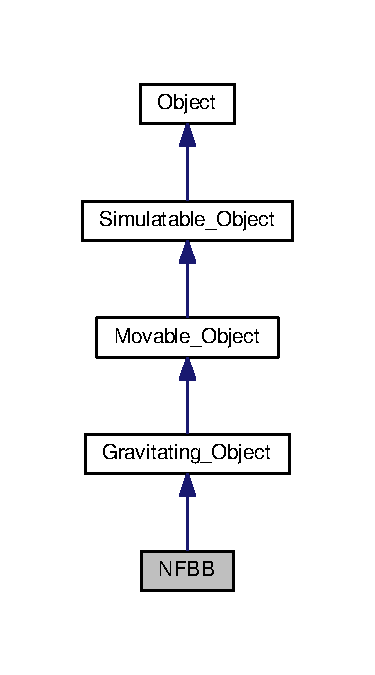
\includegraphics[width=180pt]{classNFBB__inherit__graph}
\end{center}
\end{figure}


Collaboration diagram for N\+F\+B\+B\+:\nopagebreak
\begin{figure}[H]
\begin{center}
\leavevmode
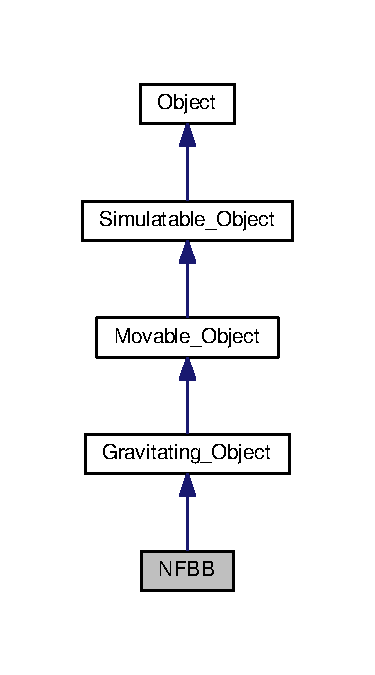
\includegraphics[width=180pt]{classNFBB__coll__graph}
\end{center}
\end{figure}
\subsection*{Public Member Functions}
\begin{DoxyCompactItemize}
\item 
\hyperlink{classNFBB_a87d7681f930eb71fd22daa8b41c8f624}{N\+F\+B\+B} (const sf\+::\+Vector2f \&, const sf\+::\+Vector2f \&, const std\+::string \&, const sf\+::\+Texture $\ast$)
\begin{DoxyCompactList}\small\item\em \char`\"{}\+Constructor\char`\"{} \end{DoxyCompactList}\item 
virtual std\+::vector$<$ \hyperlink{classObject}{Object} $\ast$ $>$ \hyperlink{classNFBB_a42a134a62a5d4049b74e7b4f4d7402dc}{simulate} (const int, const std\+::vector$<$ const \hyperlink{classObject}{Object} $\ast$ $>$ \&) overridefinal
\begin{DoxyCompactList}\small\item\em \char`\"{}\+Executes simulation of object\char`\"{} \end{DoxyCompactList}\end{DoxyCompactItemize}
\subsection*{Additional Inherited Members}


\subsection{Constructor \& Destructor Documentation}
\hypertarget{classNFBB_a87d7681f930eb71fd22daa8b41c8f624}{\index{N\+F\+B\+B@{N\+F\+B\+B}!N\+F\+B\+B@{N\+F\+B\+B}}
\index{N\+F\+B\+B@{N\+F\+B\+B}!N\+F\+B\+B@{N\+F\+B\+B}}
\subsubsection[{N\+F\+B\+B}]{\setlength{\rightskip}{0pt plus 5cm}N\+F\+B\+B\+::\+N\+F\+B\+B (
\begin{DoxyParamCaption}
\item[{const sf\+::\+Vector2f \&}]{position, }
\item[{const sf\+::\+Vector2f \&}]{size, }
\item[{const std\+::string \&}]{type, }
\item[{const sf\+::\+Texture $\ast$}]{texture}
\end{DoxyParamCaption}
)}}\label{classNFBB_a87d7681f930eb71fd22daa8b41c8f624}


\char`\"{}\+Constructor\char`\"{} 


\begin{DoxyParams}{Parameters}
{\em position} & \char`\"{}\+Position of the object\char`\"{} \\
\hline
{\em size} & \char`\"{}\+Size of the object\char`\"{} \\
\hline
{\em type} & \char`\"{}\+Type of the object\char`\"{} \\
\hline
{\em texture} & \char`\"{}\+Texture of the object\char`\"{} \\
\hline
\end{DoxyParams}


\subsection{Member Function Documentation}
\hypertarget{classNFBB_a42a134a62a5d4049b74e7b4f4d7402dc}{\index{N\+F\+B\+B@{N\+F\+B\+B}!simulate@{simulate}}
\index{simulate@{simulate}!N\+F\+B\+B@{N\+F\+B\+B}}
\subsubsection[{simulate}]{\setlength{\rightskip}{0pt plus 5cm}std\+::vector$<$ {\bf Object} $\ast$ $>$ N\+F\+B\+B\+::simulate (
\begin{DoxyParamCaption}
\item[{const int}]{simulation\+\_\+cycles, }
\item[{const std\+::vector$<$ const {\bf Object} $\ast$ $>$ \&}]{objects}
\end{DoxyParamCaption}
)\hspace{0.3cm}{\ttfamily [final]}, {\ttfamily [override]}, {\ttfamily [virtual]}}}\label{classNFBB_a42a134a62a5d4049b74e7b4f4d7402dc}


\char`\"{}\+Executes simulation of object\char`\"{} 


\begin{DoxyParams}{Parameters}
{\em simulation\+\_\+cycles} & \char`\"{}\+Number simulation\+\_\+cycles the object will be subjected this simulation-\/sequence\char`\"{} \\
\hline
{\em objects} & \char`\"{}\+Objects to check for collision with\char`\"{} \\
\hline
\end{DoxyParams}
\begin{DoxyReturn}{Returns}
\char`\"{}\+New objects spawned by this object\char`\"{} 
\end{DoxyReturn}


Reimplemented from \hyperlink{classMovable__Object_ac267e0c945b558b0cf533d7fbe5ee7c3}{Movable\+\_\+\+Object}.



The documentation for this class was generated from the following files\+:\begin{DoxyCompactItemize}
\item 
objects/non\+\_\+abstract/nfbb.\+h\item 
objects/non\+\_\+abstract/nfbb.\+cc\end{DoxyCompactItemize}

\hypertarget{classObject}{\section{Object Class Reference}
\label{classObject}\index{Object@{Object}}
}


Inheritance diagram for Object\+:\nopagebreak
\begin{figure}[H]
\begin{center}
\leavevmode
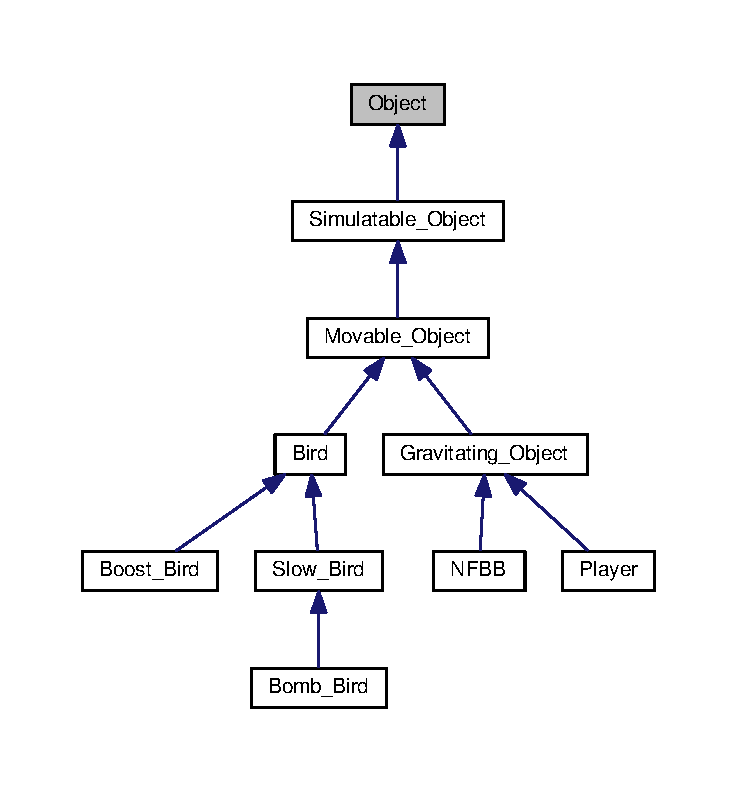
\includegraphics[width=350pt]{classObject__inherit__graph}
\end{center}
\end{figure}
\subsection*{Public Member Functions}
\begin{DoxyCompactItemize}
\item 
\hyperlink{classObject_a2df3d89d7e56659a1a0bc22d5019d587}{Object} (const sf\+::\+Vector2f \&, const sf\+::\+Vector2f \&, const std\+::string \&, const bool=false, const sf\+::\+Texture $\ast$=nullptr)
\begin{DoxyCompactList}\small\item\em \char`\"{}\+Constructor\char`\"{} \end{DoxyCompactList}\item 
\hypertarget{classObject_ad405a082a0ef9a641cd5b83ff6dd33c0}{virtual \hyperlink{classObject_ad405a082a0ef9a641cd5b83ff6dd33c0}{$\sim$\+Object} () noexcept=default}\label{classObject_ad405a082a0ef9a641cd5b83ff6dd33c0}

\begin{DoxyCompactList}\small\item\em \char`\"{}\+Virtual destrucor = default\char`\"{} \end{DoxyCompactList}\item 
std\+::string \hyperlink{classObject_a19738c1d7a0f32703a61412906edb04f}{get\+\_\+type} () const 
\item 
bool \hyperlink{classObject_ae132d029eeaaa8e3d4660951e0a35ad8}{is\+\_\+solid} () const 
\item 
bool \hyperlink{classObject_a98541d2f7380e4b5d6c805bbd7aaab01}{get\+\_\+delete\+\_\+status} () const 
\item 
sf\+::\+Rectangle\+Shape \hyperlink{classObject_a15e719bf3122cf4d8333a2b8b2f18471}{get\+\_\+shape} () const 
\begin{DoxyCompactList}\small\item\em \char`\"{}\+Returns the object's shape, which is used for drawing as well
        as getting the objects position and size\char`\"{} \end{DoxyCompactList}\end{DoxyCompactItemize}
\subsection*{Protected Attributes}
\begin{DoxyCompactItemize}
\item 
\hypertarget{classObject_a6d09f674d9c241d072a4f07934ffcac3}{const sf\+::\+Texture $\ast$ {\bfseries m\+\_\+texture}}\label{classObject_a6d09f674d9c241d072a4f07934ffcac3}

\item 
\hypertarget{classObject_a94ecef29d9e126dd4f142eb138cf93c9}{const std\+::string {\bfseries m\+\_\+type}}\label{classObject_a94ecef29d9e126dd4f142eb138cf93c9}

\item 
\hypertarget{classObject_a920a2971850ec196744477af2d7b976d}{bool {\bfseries m\+\_\+solid} \{\}}\label{classObject_a920a2971850ec196744477af2d7b976d}

\item 
\hypertarget{classObject_a122e8444050c3cc516f44be42b0aa065}{bool {\bfseries m\+\_\+delete\+\_\+status} \{\}}\label{classObject_a122e8444050c3cc516f44be42b0aa065}

\item 
\hypertarget{classObject_a4b5c1f1ad4ca0e33cdf00f74de3830f7}{sf\+::\+Rectangle\+Shape {\bfseries m\+\_\+shape}}\label{classObject_a4b5c1f1ad4ca0e33cdf00f74de3830f7}

\end{DoxyCompactItemize}


\subsection{Constructor \& Destructor Documentation}
\hypertarget{classObject_a2df3d89d7e56659a1a0bc22d5019d587}{\index{Object@{Object}!Object@{Object}}
\index{Object@{Object}!Object@{Object}}
\subsubsection[{Object}]{\setlength{\rightskip}{0pt plus 5cm}Object\+::\+Object (
\begin{DoxyParamCaption}
\item[{const sf\+::\+Vector2f \&}]{position, }
\item[{const sf\+::\+Vector2f \&}]{size, }
\item[{const std\+::string \&}]{type, }
\item[{const bool}]{solid = {\ttfamily false}, }
\item[{const sf\+::\+Texture $\ast$}]{texture = {\ttfamily nullptr}}
\end{DoxyParamCaption}
)}}\label{classObject_a2df3d89d7e56659a1a0bc22d5019d587}


\char`\"{}\+Constructor\char`\"{} 


\begin{DoxyParams}{Parameters}
{\em position} & \char`\"{}\+Position of the object\char`\"{} \\
\hline
{\em size} & \char`\"{}\+Size of the object\char`\"{} \\
\hline
{\em type} & \char`\"{}\+Type of the object\char`\"{} \\
\hline
{\em solid} & \char`\"{}\+If the object is solid\char`\"{} \\
\hline
{\em texture} & \char`\"{}\+Texture of the object\char`\"{}" \\
\hline
\end{DoxyParams}


\subsection{Member Function Documentation}
\hypertarget{classObject_a98541d2f7380e4b5d6c805bbd7aaab01}{\index{Object@{Object}!get\+\_\+delete\+\_\+status@{get\+\_\+delete\+\_\+status}}
\index{get\+\_\+delete\+\_\+status@{get\+\_\+delete\+\_\+status}!Object@{Object}}
\subsubsection[{get\+\_\+delete\+\_\+status}]{\setlength{\rightskip}{0pt plus 5cm}bool Object\+::get\+\_\+delete\+\_\+status (
\begin{DoxyParamCaption}
{}
\end{DoxyParamCaption}
) const}}\label{classObject_a98541d2f7380e4b5d6c805bbd7aaab01}
\begin{DoxyReturn}{Returns}
\char`\"{}\+If object is marked for deletion\char`\"{} 
\end{DoxyReturn}
\hypertarget{classObject_a15e719bf3122cf4d8333a2b8b2f18471}{\index{Object@{Object}!get\+\_\+shape@{get\+\_\+shape}}
\index{get\+\_\+shape@{get\+\_\+shape}!Object@{Object}}
\subsubsection[{get\+\_\+shape}]{\setlength{\rightskip}{0pt plus 5cm}sf\+::\+Rectangle\+Shape Object\+::get\+\_\+shape (
\begin{DoxyParamCaption}
{}
\end{DoxyParamCaption}
) const}}\label{classObject_a15e719bf3122cf4d8333a2b8b2f18471}


\char`\"{}\+Returns the object's shape, which is used for drawing as well
        as getting the objects position and size\char`\"{} 

\begin{DoxyReturn}{Returns}
\char`\"{}\+Shape of object\char`\"{} 
\end{DoxyReturn}
\hypertarget{classObject_a19738c1d7a0f32703a61412906edb04f}{\index{Object@{Object}!get\+\_\+type@{get\+\_\+type}}
\index{get\+\_\+type@{get\+\_\+type}!Object@{Object}}
\subsubsection[{get\+\_\+type}]{\setlength{\rightskip}{0pt plus 5cm}std\+::string Object\+::get\+\_\+type (
\begin{DoxyParamCaption}
{}
\end{DoxyParamCaption}
) const}}\label{classObject_a19738c1d7a0f32703a61412906edb04f}
\begin{DoxyReturn}{Returns}
\char`\"{}\+Type of object\char`\"{} 
\end{DoxyReturn}
\hypertarget{classObject_ae132d029eeaaa8e3d4660951e0a35ad8}{\index{Object@{Object}!is\+\_\+solid@{is\+\_\+solid}}
\index{is\+\_\+solid@{is\+\_\+solid}!Object@{Object}}
\subsubsection[{is\+\_\+solid}]{\setlength{\rightskip}{0pt plus 5cm}bool Object\+::is\+\_\+solid (
\begin{DoxyParamCaption}
{}
\end{DoxyParamCaption}
) const}}\label{classObject_ae132d029eeaaa8e3d4660951e0a35ad8}
\begin{DoxyReturn}{Returns}
\char`\"{}\+If object is solid\char`\"{} 
\end{DoxyReturn}


The documentation for this class was generated from the following files\+:\begin{DoxyCompactItemize}
\item 
objects/abstractish/object.\+h\item 
objects/abstractish/object.\+cc\end{DoxyCompactItemize}

\hypertarget{classPlayer}{\section{Player Class Reference}
\label{classPlayer}\index{Player@{Player}}
}


Inheritance diagram for Player\+:\nopagebreak
\begin{figure}[H]
\begin{center}
\leavevmode
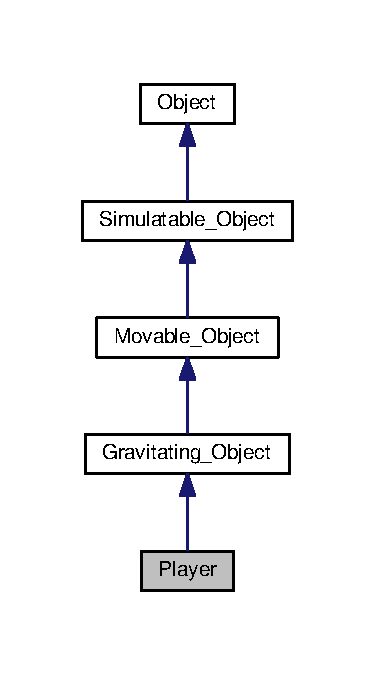
\includegraphics[width=180pt]{classPlayer__inherit__graph}
\end{center}
\end{figure}


Collaboration diagram for Player\+:\nopagebreak
\begin{figure}[H]
\begin{center}
\leavevmode
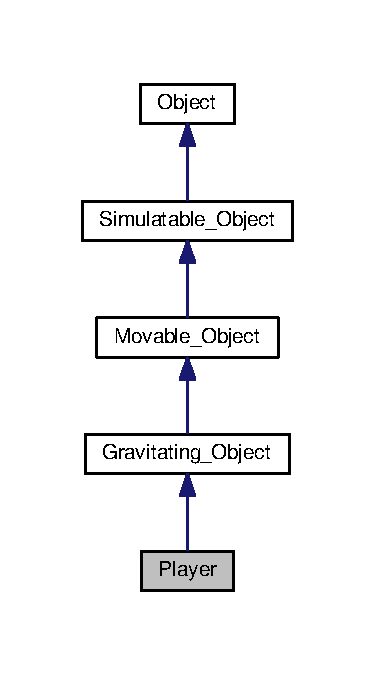
\includegraphics[width=180pt]{classPlayer__coll__graph}
\end{center}
\end{figure}
\subsection*{Public Member Functions}
\begin{DoxyCompactItemize}
\item 
\hyperlink{classPlayer_a40cd0f9599681aa40e536fc6ce47fdf2}{Player} (const sf\+::\+Vector2f \&, const sf\+::\+Vector2f \&, const std\+::string \&, const sf\+::\+Texture $\ast$, const float)
\begin{DoxyCompactList}\small\item\em \char`\"{}\+Constructor\char`\"{} \end{DoxyCompactList}\item 
virtual int \hyperlink{classPlayer_a1480bbfb767687380ad6a2bf294cdcc8}{prepare\+\_\+simulate} (const float, const float) overridefinal
\begin{DoxyCompactList}\small\item\em \char`\"{}\+Prepares simulation of object\char`\"{} \end{DoxyCompactList}\item 
const std\+::string \& \hyperlink{classPlayer_a1d89d0ff8b76784f68cf0d9e509ab242}{get\+\_\+oog\+\_\+action} () const 
\begin{DoxyCompactList}\small\item\em "Returns instructions of eventual out-\/of-\/game actions, which is used by the owning \hyperlink{classState}{State} to determine if out-\/of-\/game actions, such as quitting, should be taken" \end{DoxyCompactList}\end{DoxyCompactItemize}
\subsection*{Additional Inherited Members}


\subsection{Constructor \& Destructor Documentation}
\hypertarget{classPlayer_a40cd0f9599681aa40e536fc6ce47fdf2}{\index{Player@{Player}!Player@{Player}}
\index{Player@{Player}!Player@{Player}}
\subsubsection[{Player}]{\setlength{\rightskip}{0pt plus 5cm}Player\+::\+Player (
\begin{DoxyParamCaption}
\item[{const sf\+::\+Vector2f \&}]{position, }
\item[{const sf\+::\+Vector2f \&}]{size, }
\item[{const std\+::string \&}]{type, }
\item[{const sf\+::\+Texture $\ast$}]{texture, }
\item[{const float}]{speed}
\end{DoxyParamCaption}
)}}\label{classPlayer_a40cd0f9599681aa40e536fc6ce47fdf2}


\char`\"{}\+Constructor\char`\"{} 


\begin{DoxyParams}{Parameters}
{\em position} & \char`\"{}\+Position of the object\char`\"{} \\
\hline
{\em size} & \char`\"{}\+Size of the object\char`\"{} \\
\hline
{\em type} & \char`\"{}\+Type of the object\char`\"{} \\
\hline
{\em texture} & \char`\"{}\+Texture of the object\char`\"{} \\
\hline
{\em speed} & \char`\"{}\+Speed of the object\char`\"{} \\
\hline
\end{DoxyParams}


\subsection{Member Function Documentation}
\hypertarget{classPlayer_a1d89d0ff8b76784f68cf0d9e509ab242}{\index{Player@{Player}!get\+\_\+oog\+\_\+action@{get\+\_\+oog\+\_\+action}}
\index{get\+\_\+oog\+\_\+action@{get\+\_\+oog\+\_\+action}!Player@{Player}}
\subsubsection[{get\+\_\+oog\+\_\+action}]{\setlength{\rightskip}{0pt plus 5cm}const std\+::string \& Player\+::get\+\_\+oog\+\_\+action (
\begin{DoxyParamCaption}
{}
\end{DoxyParamCaption}
) const}}\label{classPlayer_a1d89d0ff8b76784f68cf0d9e509ab242}


"Returns instructions of eventual out-\/of-\/game actions, which is used by the owning \hyperlink{classState}{State} to determine if out-\/of-\/game actions, such as quitting, should be taken" 

\begin{DoxyReturn}{Returns}
\char`\"{}\+Return out-\/of-\/game action\char`\"{} 
\end{DoxyReturn}
\hypertarget{classPlayer_a1480bbfb767687380ad6a2bf294cdcc8}{\index{Player@{Player}!prepare\+\_\+simulate@{prepare\+\_\+simulate}}
\index{prepare\+\_\+simulate@{prepare\+\_\+simulate}!Player@{Player}}
\subsubsection[{prepare\+\_\+simulate}]{\setlength{\rightskip}{0pt plus 5cm}int Player\+::prepare\+\_\+simulate (
\begin{DoxyParamCaption}
\item[{const float}]{distance\+\_\+modifier, }
\item[{const float}]{gravity\+\_\+constant}
\end{DoxyParamCaption}
)\hspace{0.3cm}{\ttfamily [final]}, {\ttfamily [override]}, {\ttfamily [virtual]}}}\label{classPlayer_a1480bbfb767687380ad6a2bf294cdcc8}


\char`\"{}\+Prepares simulation of object\char`\"{} 


\begin{DoxyParams}{Parameters}
{\em distance\+\_\+modifier} & \char`\"{}\+Delta since last simulation-\/sequence\char`\"{} \\
\hline
{\em gravity\+\_\+constant} & \char`\"{}\+How much high the gravity is\char`\"{} \\
\hline
\end{DoxyParams}
\begin{DoxyReturn}{Returns}
\char`\"{}\+Simulation cycles required by this object this simulation-\/sequence\char`\"{} 
\end{DoxyReturn}


Reimplemented from \hyperlink{classGravitating__Object_a187404d6df6ff16a86a33a3f4a8aab85}{Gravitating\+\_\+\+Object}.



The documentation for this class was generated from the following files\+:\begin{DoxyCompactItemize}
\item 
objects/non\+\_\+abstract/player.\+h\item 
objects/non\+\_\+abstract/player.\+cc\end{DoxyCompactItemize}

\hypertarget{classSimulatable__Object}{\section{Simulatable\+\_\+\+Object Class Reference}
\label{classSimulatable__Object}\index{Simulatable\+\_\+\+Object@{Simulatable\+\_\+\+Object}}
}


Inheritance diagram for Simulatable\+\_\+\+Object\+:\nopagebreak
\begin{figure}[H]
\begin{center}
\leavevmode
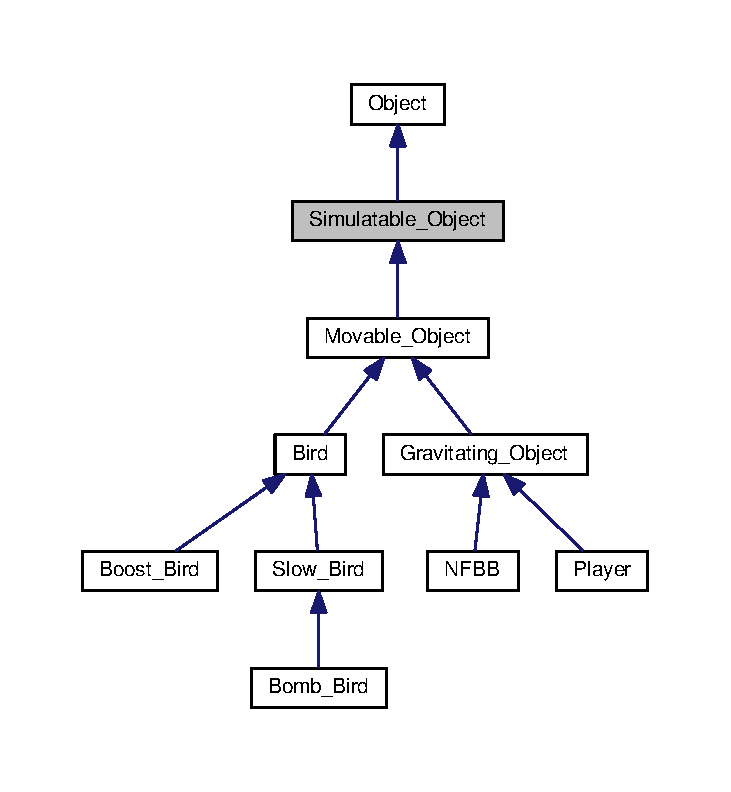
\includegraphics[width=350pt]{classSimulatable__Object__inherit__graph}
\end{center}
\end{figure}


Collaboration diagram for Simulatable\+\_\+\+Object\+:\nopagebreak
\begin{figure}[H]
\begin{center}
\leavevmode
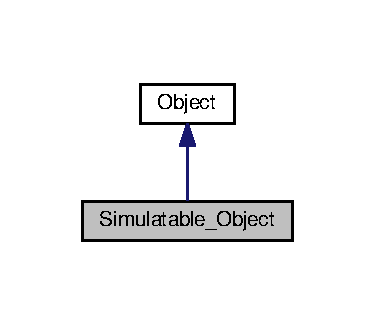
\includegraphics[width=180pt]{classSimulatable__Object__coll__graph}
\end{center}
\end{figure}
\subsection*{Public Member Functions}
\begin{DoxyCompactItemize}
\item 
\hyperlink{classSimulatable__Object_a0ca1611db5809ac78440a862ba986af7}{Simulatable\+\_\+\+Object} (const sf\+::\+Vector2f \&, const sf\+::\+Vector2f \&, const std\+::string \&, const bool=false, const sf\+::\+Texture $\ast$=nullptr)
\begin{DoxyCompactList}\small\item\em \char`\"{}\+Constructor\char`\"{} \end{DoxyCompactList}\item 
virtual int \hyperlink{classSimulatable__Object_abe7c02fe250ef5be42011890d8a7b37b}{prepare\+\_\+simulate} (const float, const float)=0
\begin{DoxyCompactList}\small\item\em \char`\"{}\+Prepares simulation of object\char`\"{} \end{DoxyCompactList}\item 
virtual std\+::vector$<$ \hyperlink{classObject}{Object} $\ast$ $>$ \hyperlink{classSimulatable__Object_a60fb2da770367330360a90afc7b724f1}{simulate} (const int, const std\+::vector$<$ const \hyperlink{classObject}{Object} $\ast$ $>$ \&)=0
\begin{DoxyCompactList}\small\item\em \char`\"{}\+Executes simulation of object\char`\"{} \end{DoxyCompactList}\item 
virtual void \hyperlink{classSimulatable__Object_a1c542c4d9cb7ba923ea9f974e5f03e84}{end\+\_\+simulate} (const std\+::vector$<$ const \hyperlink{classObject}{Object} $\ast$ $>$ \&objects)
\begin{DoxyCompactList}\small\item\em \char`\"{}\+Executes end-\/of-\/simulation logic of object\char`\"{} \end{DoxyCompactList}\end{DoxyCompactItemize}
\subsection*{Protected Member Functions}
\begin{DoxyCompactItemize}
\item 
\hypertarget{classSimulatable__Object_a2d7252861e8dea6b3bb9909421b88766}{virtual const std\+::vector\\*
$<$ const \hyperlink{classObject}{Object} $\ast$ $>$ {\bfseries get\+\_\+colliding\+\_\+objects} (const std\+::vector$<$ const \hyperlink{classObject}{Object} $\ast$ $>$ \&) const }\label{classSimulatable__Object_a2d7252861e8dea6b3bb9909421b88766}

\end{DoxyCompactItemize}
\subsection*{Additional Inherited Members}


\subsection{Constructor \& Destructor Documentation}
\hypertarget{classSimulatable__Object_a0ca1611db5809ac78440a862ba986af7}{\index{Simulatable\+\_\+\+Object@{Simulatable\+\_\+\+Object}!Simulatable\+\_\+\+Object@{Simulatable\+\_\+\+Object}}
\index{Simulatable\+\_\+\+Object@{Simulatable\+\_\+\+Object}!Simulatable\+\_\+\+Object@{Simulatable\+\_\+\+Object}}
\subsubsection[{Simulatable\+\_\+\+Object}]{\setlength{\rightskip}{0pt plus 5cm}Simulatable\+\_\+\+Object\+::\+Simulatable\+\_\+\+Object (
\begin{DoxyParamCaption}
\item[{const sf\+::\+Vector2f \&}]{position, }
\item[{const sf\+::\+Vector2f \&}]{size, }
\item[{const std\+::string \&}]{type, }
\item[{const bool}]{solid = {\ttfamily false}, }
\item[{const sf\+::\+Texture $\ast$}]{texture = {\ttfamily nullptr}}
\end{DoxyParamCaption}
)}}\label{classSimulatable__Object_a0ca1611db5809ac78440a862ba986af7}


\char`\"{}\+Constructor\char`\"{} 


\begin{DoxyParams}{Parameters}
{\em position} & \char`\"{}\+Position of the object\char`\"{} \\
\hline
{\em size} & \char`\"{}\+Size of the object\char`\"{} \\
\hline
{\em type} & \char`\"{}\+Type of the object\char`\"{} \\
\hline
{\em solid} & \char`\"{}\+If the object is solid\char`\"{} \\
\hline
{\em texture} & \char`\"{}\+Texture of the object\char`\"{}" \\
\hline
\end{DoxyParams}


\subsection{Member Function Documentation}
\hypertarget{classSimulatable__Object_a1c542c4d9cb7ba923ea9f974e5f03e84}{\index{Simulatable\+\_\+\+Object@{Simulatable\+\_\+\+Object}!end\+\_\+simulate@{end\+\_\+simulate}}
\index{end\+\_\+simulate@{end\+\_\+simulate}!Simulatable\+\_\+\+Object@{Simulatable\+\_\+\+Object}}
\subsubsection[{end\+\_\+simulate}]{\setlength{\rightskip}{0pt plus 5cm}virtual void Simulatable\+\_\+\+Object\+::end\+\_\+simulate (
\begin{DoxyParamCaption}
\item[{const std\+::vector$<$ const {\bf Object} $\ast$ $>$ \&}]{objects}
\end{DoxyParamCaption}
)\hspace{0.3cm}{\ttfamily [inline]}, {\ttfamily [virtual]}}}\label{classSimulatable__Object_a1c542c4d9cb7ba923ea9f974e5f03e84}


\char`\"{}\+Executes end-\/of-\/simulation logic of object\char`\"{} 


\begin{DoxyParams}{Parameters}
{\em objects} & \char`\"{}\+Objects to check for collision with\char`\"{}" \\
\hline
\end{DoxyParams}


Reimplemented in \hyperlink{classMovable__Object_ac9111a729082cd46a913e1877a57a930}{Movable\+\_\+\+Object}.

\hypertarget{classSimulatable__Object_abe7c02fe250ef5be42011890d8a7b37b}{\index{Simulatable\+\_\+\+Object@{Simulatable\+\_\+\+Object}!prepare\+\_\+simulate@{prepare\+\_\+simulate}}
\index{prepare\+\_\+simulate@{prepare\+\_\+simulate}!Simulatable\+\_\+\+Object@{Simulatable\+\_\+\+Object}}
\subsubsection[{prepare\+\_\+simulate}]{\setlength{\rightskip}{0pt plus 5cm}virtual int Simulatable\+\_\+\+Object\+::prepare\+\_\+simulate (
\begin{DoxyParamCaption}
\item[{const float}]{, }
\item[{const float}]{}
\end{DoxyParamCaption}
)\hspace{0.3cm}{\ttfamily [pure virtual]}}}\label{classSimulatable__Object_abe7c02fe250ef5be42011890d8a7b37b}


\char`\"{}\+Prepares simulation of object\char`\"{} 


\begin{DoxyParams}{Parameters}
{\em distance\+\_\+modifier} & \char`\"{}\+Delta since last simulation-\/sequence\char`\"{} \\
\hline
\end{DoxyParams}
\begin{DoxyReturn}{Returns}
\char`\"{}\+Simulation cycles required by this object this simulation-\/sequence\char`\"{} 
\end{DoxyReturn}


Implemented in \hyperlink{classBird_af2882ba302f03c5bdf5950cc21a39f66}{Bird}, \hyperlink{classPlayer_a1480bbfb767687380ad6a2bf294cdcc8}{Player}, and \hyperlink{classGravitating__Object_a187404d6df6ff16a86a33a3f4a8aab85}{Gravitating\+\_\+\+Object}.

\hypertarget{classSimulatable__Object_a60fb2da770367330360a90afc7b724f1}{\index{Simulatable\+\_\+\+Object@{Simulatable\+\_\+\+Object}!simulate@{simulate}}
\index{simulate@{simulate}!Simulatable\+\_\+\+Object@{Simulatable\+\_\+\+Object}}
\subsubsection[{simulate}]{\setlength{\rightskip}{0pt plus 5cm}virtual std\+::vector$<${\bf Object}$\ast$$>$ Simulatable\+\_\+\+Object\+::simulate (
\begin{DoxyParamCaption}
\item[{const int}]{, }
\item[{const std\+::vector$<$ const {\bf Object} $\ast$ $>$ \&}]{}
\end{DoxyParamCaption}
)\hspace{0.3cm}{\ttfamily [pure virtual]}}}\label{classSimulatable__Object_a60fb2da770367330360a90afc7b724f1}


\char`\"{}\+Executes simulation of object\char`\"{} 


\begin{DoxyParams}{Parameters}
{\em simulation\+\_\+cycles} & \char`\"{}\+Number simulation\+\_\+cycles the object will be subjected this simulation-\/sequence\char`\"{} \\
\hline
{\em objects} & \char`\"{}\+Objects to check for collision with\char`\"{} \\
\hline
\end{DoxyParams}
\begin{DoxyReturn}{Returns}
\char`\"{}\+New objects spawned by this object\char`\"{} 
\end{DoxyReturn}


Implemented in \hyperlink{classMovable__Object_ac267e0c945b558b0cf533d7fbe5ee7c3}{Movable\+\_\+\+Object}, \hyperlink{classBomb__Bird_a610b4c68c560a6ac30375c177642e021}{Bomb\+\_\+\+Bird}, and \hyperlink{classNFBB_a42a134a62a5d4049b74e7b4f4d7402dc}{N\+F\+B\+B}.



The documentation for this class was generated from the following files\+:\begin{DoxyCompactItemize}
\item 
objects/abstractish/simulatable\+\_\+object.\+h\item 
objects/abstractish/simulatable\+\_\+object.\+cc\end{DoxyCompactItemize}

\hypertarget{classSlow__Bird}{\section{Slow\+\_\+\+Bird Class Reference}
\label{classSlow__Bird}\index{Slow\+\_\+\+Bird@{Slow\+\_\+\+Bird}}
}


Inheritance diagram for Slow\+\_\+\+Bird\+:\nopagebreak
\begin{figure}[H]
\begin{center}
\leavevmode
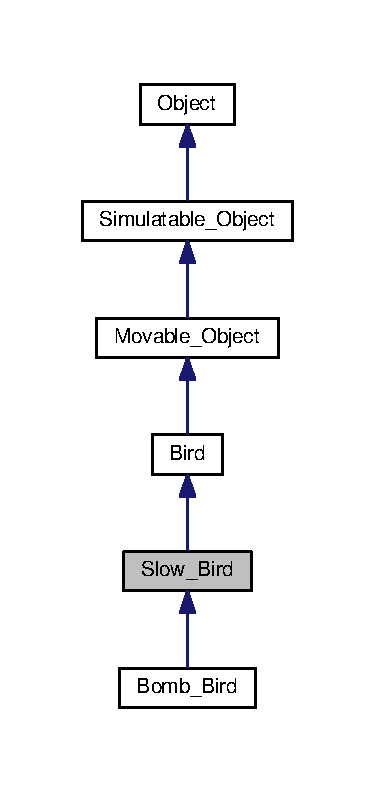
\includegraphics[width=180pt]{classSlow__Bird__inherit__graph}
\end{center}
\end{figure}


Collaboration diagram for Slow\+\_\+\+Bird\+:\nopagebreak
\begin{figure}[H]
\begin{center}
\leavevmode
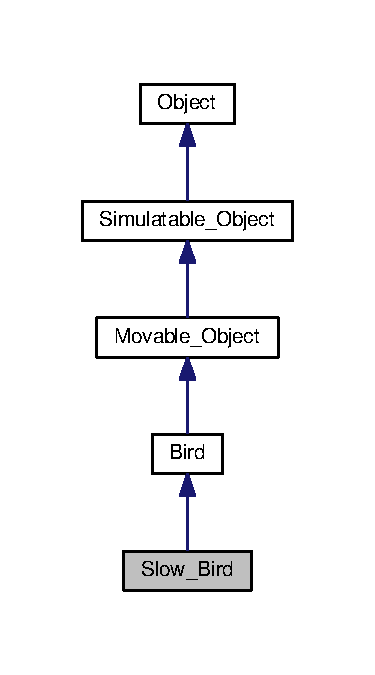
\includegraphics[width=180pt]{classSlow__Bird__coll__graph}
\end{center}
\end{figure}
\subsection*{Public Member Functions}
\begin{DoxyCompactItemize}
\item 
\hyperlink{classSlow__Bird_a52df2736474b4fe540181a43231a3f8c}{Slow\+\_\+\+Bird} (const sf\+::\+Vector2f \&, const sf\+::\+Vector2f \&, const std\+::string \&, const sf\+::\+Texture $\ast$, const float, const int)
\begin{DoxyCompactList}\small\item\em \char`\"{}\+Constructor\char`\"{} \end{DoxyCompactList}\end{DoxyCompactItemize}
\subsection*{Additional Inherited Members}


\subsection{Constructor \& Destructor Documentation}
\hypertarget{classSlow__Bird_a52df2736474b4fe540181a43231a3f8c}{\index{Slow\+\_\+\+Bird@{Slow\+\_\+\+Bird}!Slow\+\_\+\+Bird@{Slow\+\_\+\+Bird}}
\index{Slow\+\_\+\+Bird@{Slow\+\_\+\+Bird}!Slow\+\_\+\+Bird@{Slow\+\_\+\+Bird}}
\subsubsection[{Slow\+\_\+\+Bird}]{\setlength{\rightskip}{0pt plus 5cm}Slow\+\_\+\+Bird\+::\+Slow\+\_\+\+Bird (
\begin{DoxyParamCaption}
\item[{const sf\+::\+Vector2f \&}]{position, }
\item[{const sf\+::\+Vector2f \&}]{size, }
\item[{const std\+::string \&}]{type, }
\item[{const sf\+::\+Texture $\ast$}]{texture, }
\item[{const float}]{speed, }
\item[{const int}]{direction}
\end{DoxyParamCaption}
)}}\label{classSlow__Bird_a52df2736474b4fe540181a43231a3f8c}


\char`\"{}\+Constructor\char`\"{} 


\begin{DoxyParams}{Parameters}
{\em position} & \char`\"{}\+Position of the object\char`\"{} \\
\hline
{\em size} & \char`\"{}\+Size of the object\char`\"{} \\
\hline
{\em type} & \char`\"{}\+Type of the object\char`\"{} \\
\hline
{\em texture} & \char`\"{}\+Texture of the object\char`\"{} \\
\hline
{\em speed} & \char`\"{}\+Speed of the object\char`\"{} \\
\hline
{\em direction} & \char`\"{}\+Direction of the object\char`\"{} \\
\hline
{\em nfbb\+\_\+texture} & \char`\"{}\+Texture of N\+F\+B\+B-\/objects spawned by the object\char`\"{} \\
\hline
\end{DoxyParams}


The documentation for this class was generated from the following files\+:\begin{DoxyCompactItemize}
\item 
objects/non\+\_\+abstract/slow\+\_\+bird.\+h\item 
objects/non\+\_\+abstract/slow\+\_\+bird.\+cc\end{DoxyCompactItemize}

\hypertarget{classState}{\section{State Class Reference}
\label{classState}\index{State@{State}}
}


Inheritance diagram for State\+:\nopagebreak
\begin{figure}[H]
\begin{center}
\leavevmode
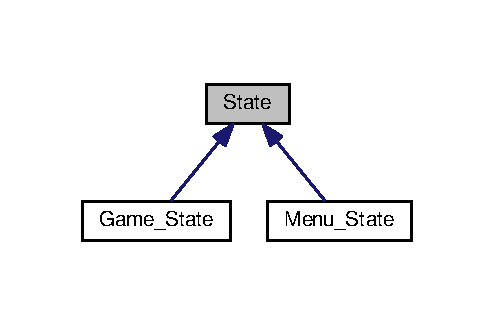
\includegraphics[width=237pt]{classState__inherit__graph}
\end{center}
\end{figure}
\subsection*{Public Member Functions}
\begin{DoxyCompactItemize}
\item 
\hypertarget{classState_a591f523d68d09675b3bd6f8e1084e642}{virtual \hyperlink{classState_a591f523d68d09675b3bd6f8e1084e642}{$\sim$\+State} () noexcept}\label{classState_a591f523d68d09675b3bd6f8e1084e642}

\begin{DoxyCompactList}\small\item\em \char`\"{}\+Virtual destructor which frees all resources owned by the state\char`\"{} \end{DoxyCompactList}\item 
\hypertarget{classState_af0cf4ef9c4b4e9a22dacf949f3df8cea}{virtual void {\bfseries prepare\+\_\+simulate} ()=0}\label{classState_af0cf4ef9c4b4e9a22dacf949f3df8cea}

\item 
\hypertarget{classState_a2fd001147b34d4a07102ba0acf680982}{virtual int {\bfseries simulate} ()=0}\label{classState_a2fd001147b34d4a07102ba0acf680982}

\item 
\hypertarget{classState_aacfda33b8dc4e6d39febdb192270a85a}{virtual void {\bfseries set\+\_\+view} (sf\+::\+View \&)=0}\label{classState_aacfda33b8dc4e6d39febdb192270a85a}

\item 
const sf\+::\+Sprite \& \hyperlink{classState_a9e132079dc08365e3c30633dd002ab8c}{get\+\_\+background} () const 
\item 
const std\+::vector$<$ const \\*
\hyperlink{classObject}{Object} $\ast$ $>$ \& \hyperlink{classState_aa234d5b01d5f75580825ea0e38074482}{get\+\_\+texturated\+\_\+objects} () const 
\item 
std\+::unordered\+\_\+map\\*
$<$ std\+::string, sf\+::\+Text $>$ \& \hyperlink{classState_a38fe48726722d318d346608f4f947121}{ref\+\_\+text\+\_\+objects} ()
\end{DoxyCompactItemize}
\subsection*{Protected Member Functions}
\begin{DoxyCompactItemize}
\item 
\hypertarget{classState_a2ebdd6e26d78ad2d34a8bf14ddb7ccf3}{virtual void \hyperlink{classState_a2ebdd6e26d78ad2d34a8bf14ddb7ccf3}{soft\+\_\+reset} ()}\label{classState_a2ebdd6e26d78ad2d34a8bf14ddb7ccf3}

\begin{DoxyCompactList}\small\item\em \char`\"{}\+Resetar statet, kan skrivas över av ärvande klasser\char`\"{} \end{DoxyCompactList}\end{DoxyCompactItemize}
\subsection*{Protected Attributes}
\begin{DoxyCompactItemize}
\item 
\hypertarget{classState_a9fe3983efbf800d94bde79b304fa0769}{std\+::unordered\+\_\+map\\*
$<$ std\+::string, sf\+::\+Texture $\ast$ $>$ {\bfseries textures}}\label{classState_a9fe3983efbf800d94bde79b304fa0769}

\item 
\hypertarget{classState_a4982a5b77746daf5e042359b45cb9a3a}{sf\+::\+Texture {\bfseries background\+\_\+texture}}\label{classState_a4982a5b77746daf5e042359b45cb9a3a}

\item 
\hypertarget{classState_addd1389225a80440a320adbb386cfe12}{sf\+::\+Sprite {\bfseries background}}\label{classState_addd1389225a80440a320adbb386cfe12}

\item 
\hypertarget{classState_ac01e57d52a3bf0d9b24c02daecd79e30}{sf\+::\+Font {\bfseries font}}\label{classState_ac01e57d52a3bf0d9b24c02daecd79e30}

\item 
\hypertarget{classState_a9f93fadc63056740b57f2b8655327fcd}{std\+::vector$<$ const \hyperlink{classObject}{Object} $\ast$ $>$ {\bfseries objects}}\label{classState_a9f93fadc63056740b57f2b8655327fcd}

\item 
\hypertarget{classState_a8f0f08cc8fcc900e4864f42d53a4d6b5}{std\+::vector$<$ const \hyperlink{classObject}{Object} $\ast$ $>$ {\bfseries texturated\+\_\+objects}}\label{classState_a8f0f08cc8fcc900e4864f42d53a4d6b5}

\item 
\hypertarget{classState_affee9f7ca66bb6a54f882b297939abbb}{std\+::unordered\+\_\+map\\*
$<$ std\+::string, sf\+::\+Text $>$ {\bfseries text\+\_\+objects}}\label{classState_affee9f7ca66bb6a54f882b297939abbb}

\end{DoxyCompactItemize}


\subsection{Member Function Documentation}
\hypertarget{classState_a9e132079dc08365e3c30633dd002ab8c}{\index{State@{State}!get\+\_\+background@{get\+\_\+background}}
\index{get\+\_\+background@{get\+\_\+background}!State@{State}}
\subsubsection[{get\+\_\+background}]{\setlength{\rightskip}{0pt plus 5cm}const sf\+::\+Sprite \& State\+::get\+\_\+background (
\begin{DoxyParamCaption}
{}
\end{DoxyParamCaption}
) const}}\label{classState_a9e132079dc08365e3c30633dd002ab8c}
\begin{DoxyReturn}{Returns}
\char`\"{}\+Returns the background set in the state\char`\"{} 
\end{DoxyReturn}
\hypertarget{classState_aa234d5b01d5f75580825ea0e38074482}{\index{State@{State}!get\+\_\+texturated\+\_\+objects@{get\+\_\+texturated\+\_\+objects}}
\index{get\+\_\+texturated\+\_\+objects@{get\+\_\+texturated\+\_\+objects}!State@{State}}
\subsubsection[{get\+\_\+texturated\+\_\+objects}]{\setlength{\rightskip}{0pt plus 5cm}const std\+::vector$<$ const {\bf Object} $\ast$ $>$ \& State\+::get\+\_\+texturated\+\_\+objects (
\begin{DoxyParamCaption}
{}
\end{DoxyParamCaption}
) const}}\label{classState_aa234d5b01d5f75580825ea0e38074482}
\begin{DoxyReturn}{Returns}
\char`\"{}\+Returns the texturated\+\_\+objects owned by the state\char`\"{} 
\end{DoxyReturn}
\hypertarget{classState_a38fe48726722d318d346608f4f947121}{\index{State@{State}!ref\+\_\+text\+\_\+objects@{ref\+\_\+text\+\_\+objects}}
\index{ref\+\_\+text\+\_\+objects@{ref\+\_\+text\+\_\+objects}!State@{State}}
\subsubsection[{ref\+\_\+text\+\_\+objects}]{\setlength{\rightskip}{0pt plus 5cm}std\+::unordered\+\_\+map$<$ std\+::string, sf\+::\+Text $>$ \& State\+::ref\+\_\+text\+\_\+objects (
\begin{DoxyParamCaption}
{}
\end{DoxyParamCaption}
)}}\label{classState_a38fe48726722d318d346608f4f947121}
\begin{DoxyReturn}{Returns}
\char`\"{}\+Returns the text\+\_\+objects owned by the state as a non-\/const reference\char`\"{} 
\end{DoxyReturn}


The documentation for this class was generated from the following files\+:\begin{DoxyCompactItemize}
\item 
states/abstract/state.\+h\item 
states/abstract/state.\+cc\end{DoxyCompactItemize}

%--- End generated contents ---

% Index
\newpage
\phantomsection
\addcontentsline{toc}{chapter}{Index}
\printindex

\end{document}
